\documentclass[final,onefignum]{siamart190516}
%\documentclass[review,onefignum]{siamart190516}

\usepackage{amssymb}
\usepackage{pgfplots,tikz}
\pgfplotsset{compat=1.15}

\newtheorem{example}{Example}

% math macros
\newcommand\bb{\mathbf{b}}
\newcommand\bbf{\mathbf{f}}
\newcommand\bG{\mathbf{G}}
\newcommand\bn{\mathbf{n}}
\newcommand\bq{\mathbf{q}}
\newcommand\br{\mathbf{r}}
\newcommand\bu{\mathbf{u}}
\newcommand\bv{\mathbf{v}}
\newcommand\bx{\mathbf{x}}
\newcommand\by{\mathbf{y}}

\newcommand\bQ{\mathbf{Q}}
\newcommand\bV{\mathbf{V}}
\newcommand\bX{\mathbf{X}}
\newcommand\bY{\mathbf{Y}}

\newcommand\CC{\mathbb{C}}
\newcommand{\DDt}[1]{\ensuremath{\frac{d #1}{d t}}}
\newcommand{\ddt}[1]{\ensuremath{\frac{\partial #1}{\partial t}}}
\newcommand{\ddx}[1]{\ensuremath{\frac{\partial #1}{\partial x}}}
\newcommand{\ddy}[1]{\ensuremath{\frac{\partial #1}{\partial y}}}
\newcommand{\ddxp}[1]{\ensuremath{\frac{\partial #1}{\partial x'}}}
\newcommand{\ddz}[1]{\ensuremath{\frac{\partial #1}{\partial z}}}
\newcommand{\ddxx}[1]{\ensuremath{\frac{\partial^2 #1}{\partial x^2}}}
\newcommand{\ddyy}[1]{\ensuremath{\frac{\partial^2 #1}{\partial y^2}}}
\newcommand{\ddxy}[1]{\ensuremath{\frac{\partial^2 #1}{\partial x \partial y}}}
\newcommand{\ddzz}[1]{\ensuremath{\frac{\partial^2 #1}{\partial z^2}}}
\newcommand{\Div}{\nabla\cdot}
\newcommand\eps{\epsilon}
\newcommand{\grad}{\nabla}
\newcommand{\ihat}{\mathbf{i}}
\newcommand{\ip}[2]{\ensuremath{\left<#1,#2\right>}}
\newcommand{\jhat}{\mathbf{j}}
\newcommand{\khat}{\mathbf{k}}
\newcommand{\nhat}{\mathbf{n}}
\newcommand\lam{\lambda}
\newcommand\lap{\triangle}
\newcommand\Matlab{\textsc{Matlab}\xspace}
\newcommand\RR{\mathbb{R}}
\newcommand\vf{\varphi}



\title{Conservation laws for free-boundary fluid layers\thanks{Draft date: \today.  Supported by NASA grant \# NNX13AM16G.}}

\author{Ed Bueler\thanks{Dept.~of Mathematics and Statistics, University of Alaska Fairbanks \,\, (\texttt{elbueler@alaska.edu}).}}

\begin{document}
\maketitle

\begin{abstract}
FIXME
\end{abstract}


\pagestyle{myheadings}
\thispagestyle{plain}
\markboth{ED BUELER}{CONSERVATION LAWS FOR FREE-BOUNDARY FLUID LAYERS}


\section{Introduction}  \label{sec:intro}

Consider a thin layer of fluid which moves.  Suppose that fluid mass can be added (accumulation, precipitation) or removed (ablation, evaporation) from the layer by external agents.  Through flow and these addition/removal processes, the thickness of the layer will change in both time and space.

We consider models of such fluid layers in which the fluid geometry is described by a nonnegative thickness function.  In such models the addition/removal processes are combined into a signed source term in a two-spatial-dimension mass conservation equation.  Supposing that the addition/removal processes are defined on a larger (supposed fixed) region, the mass conservation equation applies only in those areas where the thickness is positive.  Because the region of positive thickness, i.e.~the fluid-covered domain, changes in time, the problem of determining the fluid motion is of free-boundary type.

In physically-complete models the mass conservation equation combines with further momentum and energy conservation equations, the flow physics, which are part of how the evolution of layer geometry and state are determined.  Additionally there may be models determining the addition/removal processes, i.e.~the ``climate'' of the fluid layer, which are coupled to the fluid layer geometry.  These models combine to determine changes in the location of the free/moving boundary at which the thickness goes to zero.  This paper contains a basic, and admittedly incomplete, analysis of the mathematical well-posedness of such climate-influenced fluid layer models.  We start by extracting the minimal mathematical form which includes flow, climate, and nonnegative-thickness constraint.  After considering well-posedness we then focus on certain tradeoffs inherent in numerical solutions of such models.

Problems of this free-boundary type appear within models of glaciers and ice sheets \cite{Bueler2016,CalvoDuranyVazquez2000,Calvoetal2002,DiazSchiavi1999,EgholmNielsen2010,JouvetBueler2012},  surface and subsurface hydrology \cite{AlonsoSantillanaDawson2008,Maxwelletal2014}, and sea ice \cite{LipscombHunke2004,Thorndikeetal1975}.  Furthermore, multiphysics models can contain thin-layer and free-boundary sub-models for various species (or phases) of fluids.  For example, in comprehensive models of glaciers and ice sheets there are submodels describing floating ice shelves \cite{Albrechtetal2011}, supra- and suglacial hydrology of liquid water \cite{Aschwandenetal2012,BuelervanPelt2015,Schoofetal2012}, and sediment transport \cite{Brinkerhoffetal2017}.

In such geophysical and climate-modeling contexts, determining the fluid-covered area is a leading-order modeling goal.  For example, snow and ice are much more reflective than the substrate they cover (i.e.~land or ocean), so deciding whether grid cells are ice-covered or ice-free is a significant aspect of climate modeling.  However, conservation of mass, including precise accounting of mass transfers to and from the modeled fluid to other fluid phases, is a goal of equal importance.

The above geoscientific applications drive the author's interest, but the situation is as familiar as the dynamics of rain on a car windshield \cite{Kondic2003}.  Precipitation, evaporation, gravity, wind stresses, and surface tension all combine to determine the evolution of the geometry of the rain drops and rivulets, and of the wetted and dry domains.

If the fluid is modeled as having constant density then the (nonnegative) layer thickness can be regarded as the conserved quantity, equivalent to layer density (mass per unit area).  In models for variable density fluids the vertical integral of density is the conserved quantity in the two-dimensional conservation equations, but this variable must also be nonnegative.  As mass conservation of constant-density fluids is our primary example, for simplicity we call the conserved quantity ``mass'' and the corresponding nonnegative variable ``thickness''.

Suppose $\Omega \subset \RR^d$, $d\ge 1$, is a bounded open region with regular (Lipshitz) boundary.  (In cases of geophysical interest, $d=2$.)  Let $T>0$.  The layer thickness function $u(x,t)$, which lives in a function space addressed below, is defined for $x\in \bar\Omega$ and $t \in [0,T]$ but where there is no fluid we have $u(x,t)=0$.  The rate of flow is described by a vector flux $\bq$ and the climate (addition/removal processes) by a source term $f$; we discuss parameterizations below.  The time-dependent models we consider are usually stated in strong form, including at least a mass conservation equation and an obvious, though sometimes-unstated, inequality constraint:
\begin{align}
u_t + \Div \bq &= f &&\text{in } \Omega \times (0,T), \text{ where } u > 0 \label{eq:massconserve} \\
u &\ge 0 &&\text{in } \bar\Omega \times [0,T], \label{eq:constraint}
\end{align}
along with an initial condition $u(x,0)=u_0(x)\ge 0$.

Conservation equation \eqref{eq:massconserve} only applies where the fluid \emph{exists} ($u>0$) and not where it is \emph{absent} ($u=0$).  Constraint \eqref{eq:constraint} simply comes from the meaning of $u$ as a thickness.  The situation is pictured in Figure \ref{fig:cartoon}, where positive source values ($f>0$) are pictured as downward arrows (i.e.~as precipitation).  Evidently, well-posedness of any model including \eqref{eq:massconserve} and \eqref{eq:constraint} requires additional information about $\bq$ and $f$ along with specification of admissible functions.  We address weak formulations in Sections \ref{sec:weakform} and \ref{sec:wellposed}.

\begin{figure}[ht]
\centerline{\includegraphics[width=0.8\textwidth]{cartoon}}
\caption{Schematic of a fluid layer with a thickness $u\ge 0$.}
\label{fig:cartoon}
\end{figure}

The primary form of the flux $\bq$ considered here is local but otherwise quite general:
\begin{equation}
\bq = \bq(\grad u(x,t),u(x,t),x,t). \label{eq:fluxdepends}
\end{equation}
That flux would depend on the thickness $u$ is clear, but one reason the flux may also depend on $\grad u$ is that many of the flows under consideration are gravity-driven and viscous.  Thus the flow is at least partly diffusive, and may be written in the form $\bq=- D \grad u + (\text{other terms})$, where $D > 0$ has various dependence on $t,x,u,|\grad u|$; see \cite{Ockendonetal2003} and Subsections \ref{subsec:plap} and \ref{subsec:powertransform} below.  In other examples \eqref{eq:massconserve} is advective because we model the fluid as moving at some vertically-averaged velocity $\bX=\bX(x,t)$ determined by external factors, and have $\bq = \bX u$ (Subsection \ref{subsec:advect}).  However, our results for such advective fluxes apply even if $\bX$ comes from a (coupled) solution of a momentum conservation system, as long as it has the regularity needed to apply the theory (Subsection \ref{subsec:fluxassumptions}).  We also consider models where $\bq$ depends non-locally on the conserved quantity $u$ and its derivatives, via integrals over $\Omega$ (Subsection \ref{subsec:nonlocal}).

The ideas and results in this paper are of most interest if the \emph{source function} $f(u,x,t)$ in \eqref{eq:massconserve} takes either sign.  If $f\ge 0$ everywhere then active enforcement of constraint \eqref{eq:constraint} may not be necessary because a maximum principle can be expected to imply the nonnegativity of the solution.  By contrast, if $f<0$ in some portion of the domain then \eqref{eq:constraint} typically generates a free boundary, the location of which comes from the combined solution of \eqref{eq:massconserve} and \eqref{eq:constraint}.

The source term $f(u,x,t)$ is allowed to be nonlinear in $u$ because positive or negative feedback between layer thickness $u$ and the source $f$ occurs in certain applications (e.g.~for glaciers \cite{Jouvetetal2011}).  However, our results say nothing new about such cases and when proving well-posedness in section \ref{sec:wellposed} we simplify to the $u$-independent case $f=f(x,t)$.

Numerical approximations of these evolving fluid layers necessarily discretize time in some manner, and we only analyze the discrete-time problem.  We consider time semi-discretizations of the mass conservation equation by generally-implicit one-step methods (Section \ref{sec:strongform}).  We pose the single-time-step, continuous-space problem in weak variational form (Section \ref{sec:weakform}).  In fact Sections \ref{sec:weakform}--\ref{sec:timeseries} address the discretized-time problem independently of spatial discretization.  Section \ref{sec:spacediscretized} extends our results to a fully-discretized, unstructured finite volume/element method framework \cite{Cai1990}.

Each time-step requires the solution of a (continuous) free-boundary problem in space.  An immediate question is:
  \begin{quote}
  \renewcommand{\labelenumi}{(\roman{enumi})}
  \begin{enumerate}
  \item \emph{Is this single time-step free-boundary problem well-posed?}
  \end{enumerate}
  \end{quote}
The answer to (i) depends on the form of the flux, but by examining a weak form we can show that the answer is often ``yes,'' although sometimes subject to time-step restrictions (Section \ref{sec:wellposed}).

Our second question is less obvious but it is important in modeling practice:
  \begin{quote}
  \renewcommand{\labelenumi}{(\roman{enumi})}
  \begin{enumerate}
  \setcounter{enumi}{1}
  \item \emph{Can the discrete-time mass of the fluid layer be conserved exactly in the sense that a computable space-time integral of the source term $f$ is equal to the change in mass during a time step?}
  \end{enumerate}
  \end{quote}
By considering this question abstractly in Sections \ref{sec:timeseries} and \ref{sec:spacediscretized} we conclude that the answer is ``no,'' even in cases where the answer to (i) is ``yes.''  In general a numerical model of a fluid layer governed by \eqref{eq:massconserve} and \eqref{eq:constraint} \emph{cannot} exactly conserve mass when the free boundary moves during a time-step.

We can, however, bound and report the conservation error in a practical manner.  Such quantification of conservation errors in free-boundary models is a major purpose which guides the structure of this paper.  We first state formalism for the discretized-time problem so that sets describing the free-boundary conservation errors are precisely-defined (Sections \ref{sec:strongform}--\ref{sec:weakform}).  Later we give bounds on conservation errors in both the discretized-time (Section \ref{sec:timeseries}) and fully-discrete (Section \ref{sec:spacediscretized}) cases.

Exact discrete conservation within the fluid, i.e.~away from any free boundaries, is a common goal and property of numerical schemes \cite[and references therein]{LeVeque2002}.  When we consider fully-discretized models (Section \ref{sec:spacediscretized}) we will assume such exact discrete conservation in the interior of the fluid-covered domain.  The discrete conservation barriers we identify in this paper are entirely at the free boundary.  They are only active when the fluid layer advances, or when it retreats from areas where it was present a time-step earlier, when the source term $f$ is negative in a neighborhood of the free boundary.  In fact theoretical guidance as to achievable discrete conservation is generally absent in the literature of free-boundary fluid problems.  Reference \cite{IdelsohnOnate2010} addresses a related conservation challenge at the free surfaces of fluids but the problem is not free-boundary in the same sense.  In the context of glacier \cite{JaroschSchoofAnslow2013} and ice shelf \cite{Albrechtetal2011} modeling, for example, schemes for improved discrete mass conservation at free boundaries are proposed, but this small literature provides only \emph{ad hoc} solutions.

The mass conservation considerations and implicit time-stepping techniques of the current paper apply to sea ice models subject, however, to re-interpretation because of the manner in which mass conservation is described in such models.  They track a non-negative distribution function $g(x,t,h)$ where $h$ is the thickness dimension and $\int_0^\infty g\,dh = 1$ \cite{Thorndikeetal1975}.  Then $h$ is discretized into ``categories'' $H_{n-1} < h \le H_n$ with $H_0$ denoting the ice-free category \cite{LipscombHunke2004}.  Our results are relevant to the continuous-space equations which arise from discretizing $t$ and $h$.  Note that in such models melting is a negative source term in the evolution equation for the $H_0$ category.  Explicit updating of $g_{n,1}(x) \approx \int_{H_0}^{H_1} g(x,t_n,h)\,dh$ requires truncation (projection) to maintain nonnegativity of $g_{n,1}$.  The inequality constraint $g_{n,1} \ge 0$ is part of such a scheme whether the time-stepping is explicit or implicit.

We will see that there is no conservation error at the free boundary under the additional hypothesis that $f\ge 0$ in \eqref{eq:massconserve}.  In fact, the modeling goals of the debris flow \cite{GeorgeIverson2014} and tsunumi run-up \cite{LeVequeetal2011} literature provide a useful contrast to our concerns.  These fluid-layer problems are of free-boundary type for a hyperbolic system of mass and momentum conservation equations.  The thickness $u$ of the flow must be nonnegative, and the cited discrete models allow wet ($u>0$) and dry ($u=0$) cells.  However, the time-scales are sufficiently short (seconds to minutes) so that addition/removal sources like evaporation into the air or absorption into the ground are absent from the conservation of mass equation; $f=0$ in \eqref{eq:massconserve} in the models found in \cite{GeorgeIverson2014,LeVequeetal2011}.  The discrete-time sequence of free-boundary problems, if the model were to be formulated that way, would call for constancy of the total mass, despite the moving boundary between wet and dry areas.  In these models nonnegative fluid-layer thickness is preserved by maximum-principle properties of the discrete scheme, and exact discrete conservation applies nearly automatically.


\section{Time semi-discretization}  \label{sec:strongform}

Let $\{t_n\}_{n=0}^N$ be a sequence of increasing times with $t_0=0$ and $t_N=T>0$.  Let $\Delta t_n = t_n-t_{n-1}>0$.  Corresponding to \eqref{eq:massconserve} and \eqref{eq:constraint}, the strong form of the \emph{single time-step problem} is
\begin{align}
\frac{u_n - u_{n-1}}{\Delta t_n} + \Div \bQ_n(\grad u_n,u_n,x) &= F_n(u_n,x) &&\text{in } \Omega, \text{ where } u_n > 0 \label{eq:semimassconserve} \\
u_n &\ge 0 &&\text{in } \overline{\Omega} \label{eq:semiconstraint}
\end{align}
This problem determines a new thickness function $u_n(x) \approx u(x,t_n)$ given $u_{n-1}(x) \approx u(x,t_{n-1})$, as shown in Figure \ref{fig:timestepcartoon}.  (The weak form of the problem is given in Section \ref{sec:weakform}, but we state the strong form first because of the developed intuition of many practitioners.)

\begin{figure}[ht]
\begin{center}
\includegraphics[width=3.9in,keepaspectratio=true]{cartoon-dt}
\end{center}
\caption{The single time-step problem of \eqref{eq:semimassconserve} and \eqref{eq:semiconstraint} is a free boundary problem determining a new thickness $u_n\ge 0$ from an old thickness $u_{n-1}$, using the source term $F_n$ during the time step.}
\label{fig:timestepcartoon}
\end{figure}

A semi-discretization procedure generating equations \eqref{eq:semimassconserve} and \eqref{eq:semiconstraint}---we give several examples below---corresponds to a choice of functions
\begin{equation}
\bQ_n(\bX,v,x), \quad F_n(v,x) \label{eq:functionalforms}
\end{equation}
Here $\bX\in\RR^d$, $v\ge 0$, and $x\in \Omega$.  We will assume $\bQ_n$ is defined for all $x\in\Omega$, not just where $v(x)>0$, but that $\bQ_n(\bX,0,x)=0$, i.e.~that flux is zero for a zero-thickness layer.

\subsection{$\theta$ methods}  \label{subsec:thetamethods}  Consider a $\theta$-method discretization \cite{MortonMayers2005} of \eqref{eq:massconserve} with $0\le \theta \le 1$:
\begin{align}
  &\frac{u_n - u_{n-1}}{\Delta t_n} + \theta\, \Div \bq(\grad u_n,u_n,x,t_n) + (1-\theta) \Div \bq(\grad u_{n-1},u_{n-1},x,t_{n-1}) \label{eq:thetamethod} \\
  &\qquad =  \theta f(u_n,x,t_n) + (1-\theta) f(u_{n-1},x,t_{n-1}). \notag
\end{align}
The $\theta=0$ case is the forward Euler method, $\theta=1/2$ is trapezoid (Crank-Nicolson), and $\theta=1$ is backward Euler.  Equation \eqref{eq:thetamethod} is of form \eqref{eq:semimassconserve} with
\begin{align*}
\bQ_n(\bX,v,x) &= \theta\, \bq(\bX,v,x,t_n), \\
F_n(v,x)       &= \theta f(v,x,t_n) + (1-\theta) f(u_{n-1},x,t_{n-1}) \\
               &\qquad - (1-\theta) \Div \bq(\grad u_{n-1},u_{n-1},x,t_{n-1}).
\end{align*}

For any $\theta$ observe that the source function $F_n$ ``absorbs'' all the terms which do not involve the flux $\bq$ evaluated at time $t_n$.  If $\theta=0$ then $\bQ_n=0$; this explicit case is considered in Subsection \ref{subsec:explicit}.  On the other hand, implicitness $\theta>0$ is both helpful for the usual stability reasons \cite{MortonMayers2005} and additionally to give the smoothness needed so that the weak form of the single time-step problem can be well-posed; see Section \ref{sec:weakform}.  In the simplest implicit case of a backward Euler scheme note that $\bQ_n = \bq(\bX,v,x,t_n)$ and $F_n = f(v,x,t_n)$.

Time-discretization need not be limited to $\theta$-methods.  In particular, Appendix \ref{app:rk2} shows how multi-stage one-step schemes like Runge-Kutta can be put in form \eqref{eq:semimassconserve}.  Multi-step integration methods also fit into our framework (not shown), but the low regularity of the solution in the vicinity of the free boundary suggests that such schemes will provide no accuracy improvement.

\subsection{Associated set decomposition}  \label{subsec:setdecompose}  We can decompose $\Omega$ using the solution of problem \eqref{eq:semimassconserve} and \eqref{eq:semiconstraint}, defining three disjoint regions based on $u_n$ and $u_{n-1}$:
\begin{align*}
\Omega_n &= \left\{x \in \Omega \,\big|\, u_n(x)>0\right\}, \\
\Omega_n^r &= \left\{x \in \Omega \,\big|\, u_n(x)=0 \text{ and } u_{n-1}(x) > 0\right\}, \\
\Omega_n^0 &= \left\{x \in \Omega \,\big|\, u_n(x)=0 \text{ and } u_{n-1}(x) = 0\right\},
\end{align*}
so that
\begin{equation}
\Omega = \Omega_n \cup \Omega_n^r \cup \Omega_n^0.  \label{eq:omegadecomposition}
\end{equation}
Here the superscript ``$r$'' stands for ``retreat,'' and we call $\Omega_n^r$ the \emph{retreat set}.  Figure \ref{fig:domains} illustrates this decomposition.  If $u_n$ is continuous then $\Omega_n$ is open and sets $\Omega_n^r \cup \Omega_n^0$ and $\Omega_n^0$ are closed in $\Omega$.  (Our notation supposes that the single time-step problem is well-posed; see Section \ref{sec:wellposed}.)

\begin{figure}[ht]
\medskip
\begin{center}
\includegraphics[width=2.3in,keepaspectratio=true]{domains-fig}
\end{center}
\caption{We decompose $\Omega = \Omega_n \cup \Omega_n^r \cup \Omega_n^0$, where $\Omega_n$ is the open support of $u_n$, $\Omega_n^r$ is the retreat set, and $\Omega_n^0$ is the set on which both $u_{n-1}$ and $u_n$ are zero.}
\label{fig:domains}
\end{figure}

Assume $F_n(v,x)$ and $u_n(x)$ are continuous.  Rewriting \eqref{eq:semimassconserve} as
\begin{equation}
u_n = u_{n-1} + \Delta t_n\, F_n - \Delta t_n\, \Div \bQ_n,  \label{eq:strongflat}
\end{equation}
we see that if $u_n=0$ then the terms on the right side of \eqref{eq:strongflat} must, apparently, sum to a nonnegative number.  Furthermore, as we will assume (see \eqref{eq:Qiszero} below) that the flux of a zero-thickness layer is zero, $\bQ_n=0$ on $\Omega_n^r \cup \Omega_n^0$ where $u_n=0$.  Because also $u_{n-1}\ge 0$ and $\Delta t_n > 0$, we expect that on $\Omega_n^r \cup \Omega_n^0$ this inequality holds:
\begin{equation}
u_{n-1} + \Delta t_n\, F_n \le 0 \label{eq:strongconditionwherezero}
\end{equation}
and thus also $F_n \le 0$ on the same set.  The intuition behind \eqref{eq:strongconditionwherezero}, used below in deriving the weak form, is that the source term must be negative in a thickness-zero location where the layer was previously present (i.e.~in $\Omega_n^r$), or where it continues to be absent (in $\Omega_n^0$).


\section{Weak formulation of the single time-step problem}  \label{sec:weakform}

The strong form \eqref{eq:semimassconserve}, \eqref{eq:semiconstraint} of the single time-step problem is not adequate for mathematical progress.  PDE \eqref{eq:semimassconserve} applies only on the set $\Omega_n$ where its solution $u_n$ is positive.  Likewise, inequality \eqref{eq:strongconditionwherezero} specifies behavior on the set where $u_n=0$, and so we have posed a problem in terms of its solution.  The strong form is also inadequate because the boundary conditions satisfied by the solution $u_n$ along the free boundary $\partial\Omega_n$ are not clear.  By contrast, the weak form in this section, a variational inequality \cite{Friedman1982,KinderlehrerStampacchia1980} on a convex set of admissible functions, can be well-posed.  This formulation refers only to the set $\Omega$ and its boundary $\partial\Omega$, and not to the sets in \eqref{eq:omegadecomposition}.

We will state conditions on the discrete-time flux $\bQ_n$ (Subsection \ref{subsec:fluxassumptions}) allowing construction of a variational inequality (Subsection \ref{subsec:derivevi}) for which a sufficiently-smooth function solves the strong-form problem (subsection \ref{subsec:interior}).  Section \ref{sec:wellposed} then addresses well-posedness, which depends on properties of $\bQ_n$ that are not addressed in the current Section.

\subsection{Source and flux assumptions} \label{subsec:fluxassumptions}  Let $p\ge 1$ and recall that $L^p (\Omega)$ is the Banach space with norm $\|v\|_{L^p} = \left(\int_\Omega |v|^p\,dx\right)^{1/p}$.  The Sobolev space $W^{1,p}(\Omega)$ \cite{Evans2010} is the set of $v \in L^p(\Omega)$ satisfying $\partial_1 v,\dots,\partial_d v \in L^p(\Omega)$ and with norm
\begin{equation}
  \|v\|_{1,p} = \left(\|v\|_{L^p}^p + \sum_{i=1}^d \|\partial_i v\|_{L^p}^p\right)^{1/p}.  \label{eq:norm}
\end{equation}
If $p>d$ then $v\in W^{1,p}(\Omega)$ has a continuous representative \cite[``Morrey's inequality'']{Evans2010}, but otherwise $v$ may be discontinuous.  Denote by $W_0^{1,p}(\Omega)$ the closure of $C_c^\infty(\Omega)$ in $W^{1,p}(\Omega)$.  For $v \in W^{1,p}(\Omega)$ define $E_v = \{x\in\Omega \,\big|\, v(x) = 0\}$; note that $\grad v = 0$ a.e.~on $E_v$ \cite[lemma A.4 in chapter II]{KinderlehrerStampacchia1980}.  Also let $q=(1-1/p)^{-1}$.

Regarding the source term $F_n$, for now we assume only that if $v\in W^{1,p}(\Omega)$ then
\begin{equation}
F_n(v,x) \in L^q(\Omega).  \label{eq:FisLq}
\end{equation}

\begin{definition}  \label{ass:std}  We say $\bQ_n$ satisfies the \emph{standard flux assumptions} if
\renewcommand{\labelenumi}{\emph{\roman{enumi}})}
\begin{enumerate}
\item for each fixed $x\in \Omega$,
\begin{equation}
(\bX,z) \mapsto \bQ_n(\bX,z,x) \text{ is continuous on } \RR^d \times \RR,  \label{eq:Qiscontinuous}
\end{equation}
\item if $v \in W^{1,p}(\Omega)$ then
\begin{equation}
\bQ_n(\grad v,v,x) \in L^q(\Omega), \label{eq:QisLq}
\end{equation}
\item and
\begin{equation}
\bQ_n(\grad v,v,x)=0 \quad \text{a.e.~on } E_v. \label{eq:Qiszero}
\end{equation}
\end{enumerate}
\end{definition}

Assumptions \eqref{eq:Qiscontinuous} and \eqref{eq:QisLq} require $\bQ_n$ to be a well-behaved function.  Requirement \eqref{eq:Qiszero} says that the flux in a zero-thickness fluid layer is zero.

\subsection{Derivation of the variational inequality}  \label{subsec:derivevi}  To use the strong form in deriving a weak form we need an extra assumption that $\bQ_n$ is smooth:  For all open $S \subset \Omega$, if $v\in W^{1,p}(S)$ then
\begin{equation}
\frac{\partial}{\partial x_i} \bQ_n(\grad v,v,x) \in L^q(S). \label{eq:Qissmooth}
\end{equation}
This assumption will not affect later considerations of well-posedness (Section \ref{sec:wellposed}) or conservation errors (Sections \ref{sec:timeseries}--\ref{sec:spacediscretized}).

\begin{theorem} \label{thm:strongimpliesweak}  Suppose $u_n \in C(\overline{\Omega}) \cap W^{1,p}(\Omega)$ is a nonnegative function which solves \eqref{eq:semimassconserve} on $\Omega_n$ and \eqref{eq:strongconditionwherezero} on $\Omega_n^r \cup \Omega_n^0$.  Suppose the boundaries of the sets $\Omega_n$ and $\Omega_n^r \cup \Omega_n^0$ in decomposition \eqref{eq:omegadecomposition} are Lipschitz, and that $\overline{\Omega_n} \subset \Omega$.  Suppose $F_n$, $\bQ_n$ satisfy \eqref{eq:FisLq}, the standard flux assumptions, and \eqref{eq:Qissmooth}.  Let $\bQ = \bQ_n(\grad u_n,u_n,x)$ and $F=F_n(u_n,x)$.  Then
\begin{equation}
-\int_{\Omega} \bQ \cdot \grad(v-u_n) \ge \int_{\Omega} \left(F - \frac{u_n - u_{n-1}}{\Delta t}\right) (v-u_n) \label{eq:morallytheVI}
\end{equation}
for any $v \in C(\overline{\Omega}) \cap W^{1,p}(\Omega)$ such that $v \ge 0$.
\end{theorem}

\begin{proof}  Let $w=v-u_n$.  Using decomposition \eqref{eq:omegadecomposition} and integration by parts we get
\begin{align}
-\int_{\Omega} \bQ \cdot \grad w &= \int_{\Omega_n} (\Div \bQ) w - \int_{\partial \Omega_n} (\bQ \cdot \bn) w \label{eq:intbypartsfromstrong} \\
  &\qquad\quad + \int_{\Omega_n^r \cup \Omega_n^0} (\Div \bQ) w - \int_{\partial(\Omega_n^r \cup \Omega_n^0)} (\bQ \cdot \bn) w. \notag
\end{align}
(This needs regularity of $\partial \Omega_n$ and $\partial(\Omega_n^r \cup \Omega_n^0)$ plus assumption \eqref{eq:Qissmooth} on the sets $S=\Omega_n$ and $S=(\Omega_n^r \cup \Omega_n^0)^\circ$.)  Because $u_n$ is continuous, $u_n=0$ on $\partial \Omega_n$ and on $\partial(\Omega_n^r \cup \Omega_n^0)$.  Thus by \eqref{eq:Qiscontinuous} and \eqref{eq:Qiszero} we see that $\bQ=0$ on these boundaries, so the boundary integrals in \eqref{eq:intbypartsfromstrong} are zero.  Now, by \eqref{eq:semimassconserve} on $\Omega_n$, and by \eqref{eq:Qiszero} and \eqref{eq:Qissmooth} we have $\Div \bQ=0$ on $\Omega_n^r \cup \Omega_n^0$.  Thus we get
\begin{equation}
-\int_{\Omega} \bQ \cdot \grad w = \int_{\Omega_n} \left(F - \frac{u_n - u_{n-1}}{\Delta t}\right) w. \label{eq:equalitybeforeVI}
\end{equation}
However, by \eqref{eq:strongconditionwherezero}, $F \le 0$ on $\Omega_n^r \cup \Omega_n^0$.  Since also $u_n=0$, $u_{n-1}\ge 0$, and $w = v-u_n = v \ge 0$ on $\Omega_n^r \cup \Omega_n^0$, we have
\begin{equation}
    0 \ge \int_{\Omega_n^r \cup \Omega_n^0} \left(F - \frac{u_n - u_{n-1}}{\Delta t}\right) w. \label{eq:inequalitybeforeVI}
\end{equation}
Adding \eqref{eq:equalitybeforeVI} and \eqref{eq:inequalitybeforeVI} gives \eqref{eq:morallytheVI}.
\end{proof}

While this derivation of inequality \eqref{eq:morallytheVI} requires too many hypotheses, it adequatey motivates a weak formulation.  Inequality \eqref{eq:morallytheVI} avoids use of the solution to define subsets of $\Omega$ on which pointwise statements \eqref{eq:semimassconserve}, \eqref{eq:semiconstraint} apply.

For the following definitions, fix $p>1$ and denote $\mathcal{X} = W_0^{1,p}(\Omega)$.  Denote its dual space by $\mathcal{X}'$ and $\ip{\cdot}{\cdot}: \mathcal{X}' \times \mathcal{X} \to \RR$ for the pairing.  Note that the admissible set $\mathcal{K}$ below is a closed and convex subset of $\mathcal{X}$, and that variational inequality \eqref{eq:theVI} is the same as \eqref{eq:morallytheVI}.

\begin{definition}
\begin{equation}
\mathcal{K} = \left\{v \in \mathcal{X} \,\big|\, v(x) \ge 0\, \text{ a.e.~} x \in \Omega\right\}.  \label{eq:defineK}
\end{equation}
\end{definition}

\begin{definition}  Suppose $u_{n-1}\in\mathcal{K}$ and $\Delta t_n>0$.  Assume that $\bQ_n$ satisfies the standard flux assumptions and that $F_n$ satisfies \eqref{eq:FisLq}.  Define $A_n:\mathcal{K} \to \mathcal{X}'$ by
\begin{equation}
  \ip{A_n(v)}{\phi} = \int_\Omega \left(v - \Delta t\, F_n(v,x) - u_{n-1}\right)\phi - \Delta t_n\, \bQ_n(\grad v,v,x) \cdot \grad\phi. \label{eq:defineAn}
\end{equation}
\end{definition}

\begin{definition}  We say $u_n\in\mathcal{K}$ solves the \emph{(weak form) single time-step problem} if
\begin{equation}
  \ip{A_n(u_n)}{v-u_n} \ge 0 \quad \text{for all } v \in \mathcal{K}.  \label{eq:theVI}
\end{equation}
\end{definition}

\subsection{Interior condition}  \label{subsec:interior}  We now show a converse of Theorem \ref{thm:strongimpliesweak} which makes no regularity assumptions on the set decomposition \eqref{eq:omegadecomposition}.

\begin{theorem} \label{thm:weakimpliesstrong}  Assume $F_n$, $\bQ_n$ satisfy \eqref{eq:FisLq}, the standard flux assumptions, and \eqref{eq:Qissmooth}.  Choose $u_{n-1}\in\mathcal{K}$, and suppose that $u_n\in\mathcal{K}$ solves \eqref{eq:theVI}.  If $S \subset \Omega_n$ is open, $\overline{S}\subset \Omega$, and $u_n\in C(S)$ then \eqref{eq:semimassconserve} applies a.e.~on $S$.  If $S \subset \Omega_n^0$ is open then \eqref{eq:strongconditionwherezero} applies a.e.~on $S$.
\end{theorem}

\begin{proof}  Suppose $u_n\in\mathcal{K}$ solves \eqref{eq:theVI} and let $\bQ = \bQ_n(\grad u_n,u_n,x)$ and $F=F_n(u_n,x)$.

Suppose $S \subset \Omega_n$ is open, $\overline{S}\subset \Omega$, and $u_n\in C(S)$.  Choose any $\phi\in C_c^\infty(S)$ and extend it by zero to all of $\Omega$; note that $\phi$ can have either sign, but that $\phi=0$ on $\partial\Omega$.  Let $v = u_n + \eps \phi$ and note that $v \in \mathcal{K}$ as long as $\eps\in\RR$ is sufficiently small in magnitude.  (Specifically, if $|\eps|\le \eps_0 = \min u_n(x) / \max |\phi(x)|$, with the minimum and maximum taken over the closure of the support of $\phi$, then $v \in \mathcal{K}$.)  It follows from \eqref{eq:theVI} that
   $$\eps \int_\Omega \left(u_n - \Delta t_n\,F - u_{n-1}\right)\phi - \Delta t_n\,\bQ \cdot \grad \phi \ge 0.$$
This is true for all sufficiently-small $\eps$ and thus the integral is zero.  Integration by parts, using assumption \eqref{eq:Qissmooth} and $\phi\big|_{\partial\Omega}=0$, gives
   $$\int_\Omega \left[ u_n - \Delta t_n\,F - u_{n-1} + \Delta t_n\,\Div\bQ \right]\phi = 0.$$
Because $\phi\in C_c^\infty(S)$ is arbitrary, the quantity in square brackets is zero a.e.~on $S$.

Suppose $S \subset \Omega_n^0$ is open.  Choose any \emph{nonnegative} $\phi\in C_c^\infty(S)$, extend it by $\phi$ by zero, and let $v = u_n + \phi$ so $v\in\mathcal{K}$.  Note $u_n=0$ on the support of $\phi$.  By assumptions \eqref{eq:Qiscontinuous} and \eqref{eq:Qiszero}, $\bQ=0$ on the support of $\phi$.  Thus by \eqref{eq:theVI},
    $$0 \ge \int_{\Omega} \left(u_{n-1} + \Delta t_n\, F\right) \phi,$$
and it follows as before that $u_{n-1} + \Delta t_n\, F \le 0$ a.e.~on $S$. \end{proof}

Thus a solution of \eqref{eq:theVI} solves PDE \eqref{eq:semimassconserve} where it is positive and continuous, and where it is zero it satisfies inequality \eqref{eq:strongconditionwherezero}.  From now on we will use set decomposition \eqref{eq:omegadecomposition} only when referring to a solution $u_n$ of the weak form \eqref{eq:theVI}.


\section{Well-posedness for the single time-step problem} \label{sec:wellposed}

We show in this Section that a variety of different fluxes $\bQ_n$ yield well-posed variational inequality problems \eqref{eq:theVI}.  The \emph{a posteriori} analysis of conservation errors in Sections \ref{sec:timeseries} and \ref{sec:spacediscretized} below assumes that these problems are well-posed.

Techniques for proving well-posedness of variational inequalities in Banach spaces are relatively well-established for linear and some nonlinear elliptic problems, especially for monotone operators \cite{KinderlehrerStampacchia1980}.  We recall these tools in subsection \ref{subsec:mono} assuming the source term $F_n$ is solution-independent.  Then in the next four subsections we prove existence and uniqueness of the solution to problem \eqref{eq:theVI} for the following flux cases:
\begin{itemize}
\item[\ref{subsec:plap}] $p$-Laplacian-type parabolic (diffusion) for $1<p<\infty$,
\item[\ref{subsec:powertransform}] doubly-nonlinear parabolic, including porous media,
\item[\ref{subsec:advect}] linear advective, with a small parabolic diffusion term, and
\item[\ref{subsec:nonlocal}] linear and non-local (computed by integrals over $\Omega$).
\end{itemize}
These subsections only use the backward Euler time-stepping discretization.  At the end, subsection \ref{subsec:explicit} shows that if time-stepping is explicit or semi-explicit then regularity issues generally block the continuous-space single time-step problems from being well-posed.

\subsection{Monotone variational inequalities} \label{subsec:mono}  Recall $\mathcal{K}$ is defined in \eqref{eq:defineK}.  The following definitions can be found in \cite{KinderlehrerStampacchia1980}.  A mapping $A : \mathcal{K} \to \mathcal{X}'$ is \emph{monotone} if
\begin{equation}
   \ip{A(u) - A(v)}{u-v} \ge 0  \label{eq:monodef}
\end{equation}
for all $u,v\in\mathcal{K}$, and \emph{strictly monotone} if equality in \eqref{eq:monodef} additionally implies $u=v$.  Mapping $A$ is \emph{coercive} if there is $\phi\in \mathcal{K}$ so that
\begin{equation}
   \lim_{\|u\|\to\infty} \frac{\ip{A(u) - A(\phi)}{u-\phi}}{\|u-\phi\|} = +\infty, \label{eq:coercivedef}
\end{equation}
where the limit is taken over $u\in\mathcal{K}$.  Mapping $A : \mathcal{K} \to \mathcal{X}'$ is \emph{continuous on finite-dimensional subspaces} if for each finite-dimensional subspace $\mathcal{M} \subset \mathcal{X}$, the restriction $A : \mathcal{K}\cap \mathcal{M} \to \mathcal{X}'$ is weakly-continuous.

The theory of monotone variational inequalities in Banach spaces \cite[chapter III]{KinderlehrerStampacchia1980} says that a solution to the variational inequality
\begin{equation}
    \ip{A(u)}{v-u} \ge 0 \quad \text{for all $v\in\mathcal{K}$}, \label{eq:VIabstract}
\end{equation}
exists and is unique if $A$ is strictly monotone, coercive, and continuous on finite-dimensional subspaces.  (Note strict monotonicity alone suffices for uniqueness.)

Now consider variational inequality \eqref{eq:theVI} with $A_n$ defined by \eqref{eq:defineAn}.  It is easy to show the following lemma.

\begin{lemma}  \label{lem:continuous}  Assume \eqref{eq:Qiscontinuous} for $\bQ_n$ and that $F_n(v,x)\in L^q$ is continuous in $v$.  The map $A_n$ is continuous on finite-dimensional subspaces.
\end{lemma}

%\begin{proof} Choose $\{v_i\}_{i=1}^m \subset \mathcal{K}$ and let $\mathcal{M}=\operatorname{span}\left<v_i\right>$, a subspace of $\mathcal{X}$.  Fix $\phi\in\mathcal{X}$.  The map $g:\RR^m \to \RR$ defined by
%\begin{equation}
%  g(c_1,\dots,c_m) = \ip{A_n\left(\sum_{i=1}^m c_i v_i\right)}{\phi}
%\end{equation}
%is continuous because of \eqref{eq:Qiscontinuous} and the continuity of $F_n$.
%\end{proof}

Now we want to relate the properties of the flux $\bQ_n$ to the monotonicity and coercivity of $A_n$.  The following calculation applies when $F_n=F_n(x)$, i.e.~when the source function $F_n(v,x)$ is independent of the thickness $v$:
\begin{align}
   &\ip{A_n(u) - A_n(v)}{u-v}  \label{eq:AtoQcalculation} \\
   &\qquad = \int_\Omega (u-v)^2 - \Delta t\, \left[\bQ_n(\grad u,u,x) - \bQ_n(\grad v,v,x)\right] \cdot \grad(u-v).  \notag
\end{align}
The proof of the following lemma is therefore easy and omitted.  Note that $W^{1,p}(\Omega) \subset L^2(\Omega)$ if either $p>d$ or $d\le 2$ \cite[theorems 5.6.2 and 5.6.5]{Evans2010}.  % FIXME: check for 2nd edition.
In considering this lemma the reader should observe that in cases where $\bQ_n(\grad u,u,x)$ is proportional to $\grad u$ we expect, for physical reasons, that the flux $\bQ_n$ points generally in the direction of the negative of $\grad u$, as otherwise PDE \eqref{eq:massconserve} would behave like the ill-posed backward heat equation.

\begin{lemma}  \label{lem:monotonecoercive}  Suppose $W^{1,p}(\Omega) \subset L^2(\Omega)$.  Suppose \eqref{eq:QisLq} and that $F_n=F_n(x) \in L^q(\Omega)$.  Then
\renewcommand{\labelenumi}{(\roman{enumi})}
\begin{enumerate}
\item  $A_n$ is monotone if there is $C\le 1$ so that
\begin{equation}
\int_\Omega \left[\bQ_n(\grad u,u,x) - \bQ_n(\grad v,v,x)\right] \cdot \grad(u-v) \le \frac{C}{\Delta t_n} \|u-v\|_{L^2}^2 \label{eq:Qnmonotone}
\end{equation}
for all $u,v \in \mathcal{K}$.
\item  $A_n$ is strictly-monotone if \eqref{eq:Qnmonotone} holds with $C<1$,
\item  $A_n$ is coercive and strictly-monotone if there is $c>0$ and $r>1$ so that
\begin{equation}
\int_\Omega \left[\bQ_n(\grad u,u,x) - \bQ_n(\grad v,v,x)\right] \cdot \grad(u-v) \le - c \|u-v\|^r \label{eq:Qncoercive}
\end{equation}
for all $u,v \in \mathcal{K}$.
\end{enumerate}
\end{lemma}

Note that the right side of \eqref{eq:Qncoercive} uses the norm in $W^{1,p}(\Omega)$.  Inequality \eqref{eq:Qncoercive} implies \eqref{eq:Qnmonotone} with $C=0$, so \eqref{eq:Qncoercive} implies strict-monotonicity for $A_n$ independent of $\Delta t_n$.  Observe that \eqref{eq:Qnmonotone} is necessary and sufficient for monotonicity of $A_n$, while \eqref{eq:Qncoercive} is only sufficient for coercivity.  (For example, if the right side of \eqref{eq:Qncoercive} were instead $- c \|u-v\| \log \|u-v\|$ then $A_n$ would be coercive.)  Corollary III.1.8 of \cite{KinderlehrerStampacchia1980} now gives the following theorem.

\begin{theorem}  \label{thm:monowellposed}  Suppose $W^{1,p}(\Omega) \subset L^2(\Omega)$.  Suppose $\bQ_n$ satisfies the standard flux assumptions and that $F_n=F_n(x)\in L^q(\Omega)$.  If \eqref{eq:Qncoercive} holds for $\bQ_n$ then the single time-step weak problem \eqref{eq:theVI} has a unique solution $u\in\mathcal{K}$.
\end{theorem}

\subsection{$p$-Laplacian fluxes} \label{subsec:plap}  We can apply Lemma \ref{lem:monotonecoercive} and Theorem \ref{thm:monowellposed} to show well-posedness in certain linear and non-linear parabolic cases, that is, wherein $\bq$ has the direction of $-\grad u$.  Consider the $p$-Laplacian \cite{Evans2010} flux
\begin{equation}
  \bQ_n(\grad u) = - k |\grad u|^{p-2} \grad u \label{eq:plapflux}
\end{equation}
with $k>0$ and $1<p<\infty$, so that $\bQ_n$ satisfies the standard flux assumptions.  Formula \eqref{eq:plapflux} includes the Fourier flux as the $p=2$ case.  For the proofs in this subsection we assume $F_n=F_n(x)$ is independent of $u$, and we use inequalities from Appendix \ref{app:pinequalities}.

If $p\ge 2$ then by \eqref{eq:pbiginequality} and \eqref{eq:poincare} there is $C=C(\Omega,p)$ so that
\begin{align}
\int_\Omega \left(\bQ_n(\grad u) - \bQ_n(\grad v)\right)\cdot (\grad u - \grad v) &= -k  \int_\Omega \left(|\grad u|^{p-2} \grad u - |\grad v|^{p-2} \grad v\right)\cdot (\grad u - \grad v) \notag \\
  &\le - \frac{k}{2^{p-2}} \int_\Omega |\grad u - \grad v|^p \le - \frac{k}{C 2^{p-2}} \|u-v\|^p \label{eq:plapQnmono}
\end{align}
and thus \eqref{eq:Qncoercive} holds with $r=p$.  However, if  $1<p<2$ then we have to work harder.  Showing coercivity is possible, though not via condition \eqref{eq:Qncoercive}.  Using \eqref{eq:psmallinequality}, \eqref{eq:smallpbound}, and \eqref{eq:poincare} gives
\begin{align*}
\ip{A_n(u) - A_n(v)}{u-v} &= \|u-v\|_{L^2(\Omega)}^2 + \Delta t_n\,k \int_\Omega \left(|\grad u|^{p-2} \grad u - |\grad v|^{p-2} \grad v\right)\cdot (\grad u - \grad v) \\
  &\ge \|u-v\|_{L^2(\Omega)}^2 + \Delta t_n\,k (p-1) \int_\Omega \frac{|\grad u - \grad v|^2}{\left(|\grad u|+|\grad v|\right)^{2-p}} \\
  &\ge \|u-v\|_{L^2(\Omega)}^2 + \Delta t_n\,k (p-1) \frac{\|\grad u - \grad v\|_{L^p(\Omega; \RR^d)}^2}{\big\||\grad u|+|\grad v|\big\|_{L^p(\Omega)}^{2-p}} \\
  &\ge \|u-v\|_{L^2(\Omega)}^2 + B\, \frac{\|u - v\|^2}{\big\||\grad u|+|\grad v|\big\|_{L^p(\Omega)}^{2-p}}
\end{align*}
where $B = \Delta t_n\,k (p-1) C(\Omega,p)^{-2/p} >0$.  This shows $\ip{A_n(u) - A_n(v)}{u-v} \ge \|u-v\|_{L^2(\Omega)}^2$, so that $A_n$ is strictly-monotone.  Therefore, fixing $v$ such that $\|\grad v\|_{L^p(\Omega;\RR^d)} >0$, we have
\begin{equation*}
\frac{\ip{A_n(u) - A_n(v)}{u-v}}{\|u-v\|} \ge B\, \frac{\|u - v\|}{\big\||\grad u|+|\grad v|\big\|_{L^p(\Omega)}^{2-p}} \to \infty
\end{equation*}
as $\|u\|\to\infty$ because $0<2-p<1$, so $A_n$ is coercive.  The following Theorem is proven.

\begin{theorem}  \label{thm:plapwellposed}  If $\Omega\subset \RR^d$ is bounded, $1<p<\infty$, $F_n=F_n(x)$ is independent of $u$, and $\bQ_n$ is given by \eqref{eq:plapflux} with $k>0$, then for any $\Delta t_n>0$, \eqref{eq:theVI} has a unique solution $u\in\mathcal{K}$.
\end{theorem}

\subsection{Doubly-nonlinear fluxes} \label{subsec:powertransform}  Now consider the doubly-nonlinear flux
\begin{equation}
  \bQ_n(\grad u,u) = - k u^r |\grad u|^{p-2} \grad u \label{eq:doubleflux}
\end{equation}
where $k>0$, $r\ge 0$, and $1<p<\infty$.  This includes, as the $r=0$ case, the $p$-Laplacian \eqref{eq:plapflux}, but it also includes the porous medium equation \cite{Vazquez2007}, where $p=2$, $r=\gamma-1$, and $\bQ_n = - \tilde k \grad(u^\gamma)$.  Flux for the diffusive shallow water equations \cite{AlonsoSantillanaDawson2008} has nontrivial powers $1<r<2$ and $1<p\le 2$.  The flat-bed shallow ice approximation \cite{Calvoetal2002} flux uses $r=n+2$ and $p=n+1$ for $n>1$.

Leaving the function space undetermined for a moment, suppose we apply a power transformation $u = w^m$ where $m = (p-1)/(r+p-1)$ \cite{Raviart1970} so that $0 < m \le 1$.  Straightforward calculation turns \eqref{eq:doubleflux} into
\begin{equation}
	\bQ_n = - K |\grad w|^{p-2} \grad w, \label{eq:doublenewflux}
\end{equation}
with $K=k m^{p-1}>0$, giving the $p$-Laplacian flux \eqref{eq:plapflux}.  This transformation converts PDE \eqref{eq:semimassconserve} into a $p$-Laplacian equation with additional zeroth-order terms, namely
\begin{equation}
    - \Div\left(K|\grad w|^{p-2} \grad w\right) + G(w,x) = 0  \label{eq:doubleplap}
\end{equation}
with $G(w,x) = w^m - \Delta t_n\, F_n(w^m,x) - u_{n-1}$.  Note that in the porous media case $p=2$, equation \eqref{eq:doubleplap} is semilinear \cite{Evans2010}.

Define $\mathcal{X} = W_0^{1,p}(\Omega)$ and admissible functions $\mathcal{K}\subset \mathcal{X}$ just as in section \ref{sec:weakform}.  Define $A_n: \mathcal{K} \to \mathcal{X}'$ by
\begin{equation}
\ip{A_n(w)}{\phi} = \int_\Omega \Delta t_n\, K |\grad w|^{p-2} \grad w\cdot \grad \phi + G(w,x)\phi. \label{eq:doubleform}
\end{equation}
The weak formulation of \eqref{eq:doubleplap} is precisely \eqref{eq:VIabstract} with $A=A_n$.  The following Theorem uses the argument in subsection III.3 of \cite{KinderlehrerStampacchia1980}.

\begin{theorem}
Let $1<p<\infty$ and $r\ge 0$.  Define $m = (p-1)/(r+p-1)$.  Suppose $G(w,x)=w^m - \Delta t_n\, F_n(w^m,x) - u_{n-1}$ is in $\mathcal{X}'$ for all $w\in\mathcal{K}$, and that $G$ is nondecreasing in $w$.  Then $A_n$ in \eqref{eq:doubleform} is strictly monotone and coercive, and thus \eqref{eq:theVI} has a unique solution $u\in\mathcal{K}$.
\end{theorem}

\begin{proof}
Suppose $p\ge 2$.  If $w,v\in\mathcal{X}$ then by \eqref{eq:pbiginequality} and Poincare inequality \eqref{eq:poincare},
\begin{align*}
\ip{A_n(w)-A_n(v)}{w-v} &= \int_\Omega \Delta t_n\, K \left(|\grad w|^{p-2} \grad w - |\grad v|^{p-2} \grad v\right) \cdot \grad (w-v) \\
  &\qquad\qquad + \left(G(w,x) - G(v,x)\right) (w-v) \\
  &\ge \frac{\Delta t_n\,K}{2^{p-2}} \int_\Omega |\grad (w-v)|^p + 0 \ge \frac{\Delta t_n\,K}{2^{p-2}\, C(\Omega,p)} \|w-v\|^p.
\end{align*}
The case $1<p<2$ follows by a trivial modification of the argument in Theorem \ref{thm:plapwellposed}.
\end{proof}

\subsection{Advection by a differentiable velocity field} \label{subsec:advect}  The flux in applications such as ice shelves or sea ice is often understood to be mostly-advective (hyperbolic).  In such applications the velocity arises from solving a momentum balance, but here we simply assume the layer is transported by a differentiable velocity field $\bX \in W^{1,\infty}(\Omega;\RR^d)$,
\begin{equation}
  \bQ_n(u,x) = \bX(x) u. \label{eq:advectflux}
\end{equation}
If $1<p<\infty$ then $\bQ_n$ satisfies the standard flux assumptions on $W^{1,p}(\Omega)$.

Suppose $u,v\in\mathcal{K}$.  Noting $u=v=0$ on $\partial \Omega$, integration-by-parts shows
\begin{align}
   &\int_\Omega \left[\bQ_n(u,x) - \bQ_n(v,x)\right] \cdot \grad (u - v) = \int_\Omega \bX (u-v) \cdot \grad (u - v)   \label{eq:advectQnmono} \\
   &\qquad\qquad = \frac{1}{2}\,\int_\Omega \bX \cdot \grad\left[ (u - v)^2 \right] = - \frac{1}{2}\,\int_\Omega \left(\Div\bX\right) (u - v)^2. \notag
\end{align}
Equation \eqref{eq:advectQnmono} can be exploited in a couple of ways.  If the vector field is divergent $\Div\bX\ge 0$ then \eqref{eq:Qnmonotone} applies with $C=0$ and so $A_n$ is strictly monotone.  Otherwise, \eqref{eq:Qnmonotone} applies with $C = \frac{1}{2}\Delta t_n\,\|(\Div\bX)_{-}\|_{L^\infty(\Omega)}$, and then $A_n$ is monotone if $C \le 1$ (strictly if $C < 1$).

Consider the operator $A_n$ defined by \eqref{eq:defineAn}, as an operator from $\mathcal{K} \subset \mathcal{X} = W_0^{1,p}(\Omega)$ to the dual $\mathcal{X}'$, using flux \eqref{eq:advectflux}.  There is no reason to suppose this operator is coercive.  However, if we add a bit of diffusion in the form of a $p$-Laplacian leading-order term with coefficient $\eps>0$ and $p\ge 2$, namely
\begin{equation}
  \bQ_n(\grad u,u,x) = -\eps |\grad u|^{p-2} \grad u + \bX(x) u,   \label{eq:plapadvectflux}
\end{equation}
then the corresponding operator $A_n$ on $W_0^{1,p}(\Omega)$ is coercive.  In fact, combining \eqref{eq:plapQnmono} and \eqref{eq:advectQnmono} gives
\begin{equation}
\int_\Omega \left[\bQ_n(u,x) - \bQ_n(v,x)\right] \cdot \grad (u - v) \le - \eps c_0 \|u-v\|^p - \frac{1}{2} \int_\Omega (\Div\bX) (u-v)^2
\end{equation}
where $c_0=2^{2-p}/C(\Omega,p)>0$.  Thus
\begin{equation}
\ip{A_n(u) - A_n(v)}{u-v} \ge \eps c_0 \Delta t_n\, \|u-v\|^p + \frac{\Delta t_n}{2} \int_\Omega (\Div\bX) (u-v)^2 + \|u-v\|_{L^2(\Omega)}^2.
\end{equation}
This proves the following theorem:

\begin{theorem}  \label{thm:plapadvectwellposed}  Suppose $\bQ_n$ is given by \eqref{eq:plapadvectflux} with $\eps>0$.  If $\bX \in W^{1,\infty}(\Omega;\RR^d)$, $F_n=F_n(x)$ is independent of $u$, and $p\ge 2$, then \eqref{eq:theVI} has a unique solution $u\in\mathcal{K}$ if either $\Div \bX \ge 0$ or
\begin{equation}
  \Delta t_n \le \frac{2}{\|(\Div \bX)_-\|_{L^\infty(\Omega)}}. \label{eq:plapadvectdtcond}
\end{equation}
\end{theorem}

A bound on the product of $\Delta t_n$ and a norm of $\bX$ may be regarded as a CFL-type condition \cite{LeVeque2002}, but here the bound measures the \emph{convergence} of the velocity field and not the velocity magnitude.  If the measure of convergence $\|(\Div \bX)_-\|_{L^\infty(\Omega)}$ is small then large time steps are well-posed.  Also observe that condition \eqref{eq:plapadvectdtcond} is independent of $\eps>0$, suggesting that the pure advection problem ($\eps = 0$) may also be well-behaved.

\subsection{Non-local dependence through an integral kernel} \label{subsec:nonlocal}   The examples so far compute the flux $\bQ_n$ at $x\in\Omega$ using only the values $u(x)$ and $\grad u(x)$.  However, the flux in realistic models often comes from solving another differential equation, generally a momentum conservation equation, which is coupled to the mass-conservation equation \eqref{eq:massconserve}.  Therefore we consider fluxes that are non-local functions of the thickness $u$ and its spatial derivatives, but again for analytical simplicity we restrict to the case where $\bQ_n$ is linear in $u$.

Let $\mathcal{X} = W_0^{1,2}(\Omega)$, a Hilbert space, and let $\mathcal{K}=\{u\in\mathcal{X}|u\ge 0\}$.  Suppose $G_1(x,y)$, \dots, $G_d(x,y)$ and $K(x,y)$ are scalar, real-valued functions in $L^2(\Omega\times \Omega)$.  Define
\begin{equation}
\bQ_n[\grad u,u](x) = \int_\Omega \bG(x,y) u(y)\,dy - \int_\Omega K(x,y) \grad u(y)\,dy, \label{eq:nonlocaldefQn}
\end{equation}
where $\bG(x,y) = (G_1(x,y), \dots, G_d(x,y))$ is an $\RR^d$-valued function.  Square-bracket notation ``$\bQ_n[\cdot]$'' emphasizes general, not point-wise, dependence on $u$.  With flux \eqref{eq:nonlocaldefQn}, equation \eqref{eq:semimassconserve} is no longer a PDE, but rather a linear integro-differential equation.

Let $A_n:\mathcal{K} \to \mathcal{X}'=\mathcal{X}$ be defined by \eqref{eq:defineAn}, with $\bQ_n$ in \eqref{eq:nonlocaldefQn} as the flux, so that
\begin{align}
    \ip{A_n(v)}{\phi} &= \int_\Omega \bigg[(v - \Delta t_n\,F_n - u_{n-1})\phi - \Delta t_n\,\left(\int_\Omega \bG(x,y) v(y)\,dy\right)\cdot \grad \phi \label{eq:nonlocaldefnAn} \\
                      &\qquad\qquad + \Delta t_n\,\left(\int_\Omega K(x,y) \grad v(y)\,dy\right)\cdot \grad \phi\,\bigg]. \notag
\end{align}

Regarding the next proof, observe that two applications of Cauchy-Schwarz yield
\begin{equation}
\left|\int_\Omega \int_\Omega \bG(x,y) \cdot \grad \phi(x)\,\phi(y) \,dx\,dy\right|
  \le \|\bG\|_{L^2(\Omega\times\Omega;\RR^d)} \|\phi\|^2,   \label{eq:nonlocalGbound}
\end{equation}
where, by definition, $\|\bG\|_{L^2(\Omega\times\Omega;\RR^d)} = \left(\sum_{i=1}^d \left\|G_i\right\|_{L^2(\Omega \times \Omega)}^2\right)^{1/2}$.

\begin{theorem}  \label{thm:nonlocalwellposed}  Suppose $C(\Omega,p)$ is the Poincar\'e constant in \eqref{eq:poincare}.  Suppose $F_n=F_n(x) \in L^2(\Omega)$ is independent of $u$.  Assume $G_i \in L^2(\Omega\times\Omega)$ for $i=1,\dots,d$.  Suppose $K \in L^2(\Omega\times\Omega)$ positive and bounded below \cite{PorterStirling1990} in the sense that there is $\delta>0$ so that
\begin{equation}
   \int_\Omega \int_\Omega K(x,y) \phi(x) \phi(y)\,dx\,dy \ge \delta \|\phi\|_{L^2(\Omega)}^2 \qquad \text{for all } \phi \in L^2(\Omega).  \label{eq:nonlocalKpos}
\end{equation}
If either $\bG=0$ or
\begin{equation}
  \Delta t_n < \frac{\delta}{C(\Omega,p)\, \|\bG\|_{L^2(\Omega\times\Omega;\RR^d)}}  \label{eq:nonlocaldtcond}
\end{equation}
then $A_n$ defined by \eqref{eq:nonlocaldefnAn} is coercive and strictly monotone, and thus variational inequality \eqref{eq:theVI} has a unique solution $u\in\mathcal{K}$.
\end{theorem}

\begin{proof}  Let $\phi=u-v$ for $u,v\in\mathcal{K}$.  By \eqref{eq:nonlocalGbound}, \eqref{eq:nonlocalKpos}, and \eqref{eq:poincare},
\begin{align*}
\ip{A_n(u)-A_n(v)}{\phi} &\ge \|\phi\|_{L^2(\Omega)}^2 - \Delta t_n\,\int_\Omega \int_\Omega \bG(x,y) \cdot \grad \phi(x) \phi(y)\,dx\,dy \\
    &\qquad + \Delta t_n\,\int_\Omega \int_\Omega K(x,y) \grad \phi(x) \cdot \grad \phi(y)\,dx\,dy \\
    &\ge \|\phi\|_{L^2(\Omega)}^2 - \Delta t_n\,\|\bG\|_{L^2(\Omega\times\Omega;\RR^d)} \|\phi\|^2 + \delta \|\grad\phi\|_{L^2(\Omega;\RR^d)}^2 \\
    &\ge \|\phi\|_{L^2(\Omega)}^2 + \left(\frac{\delta}{C(\Omega,p)} - \Delta t_n\,\|\bG\|_{L^2(\Omega\times\Omega;\RR^d)}\right) \|\phi\|^2.
\end{align*}
The result follows from condition \eqref{eq:nonlocaldtcond} and definition \eqref{eq:coercivedef}.
\end{proof}

In a certain sense Theorems \ref{thm:plapadvectwellposed} and \ref{thm:nonlocalwellposed} take different approaches.  In the former the velocity $\bX$ was assumed to be differentiable and an integration-by-parts gave a criterion for well-posedness via a bound on $\Delta t$ using derivatives of $\bX$.  By contrast, in theorem \ref{thm:nonlocalwellposed} we assume only that $\bG$ is integrable, no integration-by-parts is attempted, and $\Delta t$ is bounded using the norm of $\bG$ itself.

\subsection{Explicit time-steps} \label{subsec:explicit}  Recall the explicit case of equation \eqref{eq:thetamethod}, with $\theta=0$.  In weak form the problem is variational inequality \eqref{eq:theVI}, but with $\bQ_n=0$ and
\begin{equation}
F_n = - \Div \bq(\grad u_{n-1},u_{n-1},x) + f(u_{n-1},x).  \label{eq:Fnformexplicit}
\end{equation}
One seeks $u\in\mathcal{K} \subset \mathcal{X}$ so that
\begin{equation}
\ip{A_n(u)}{\phi} = \int_\Omega (u - \Delta t_n\,F_n - u_{n-1})\phi \ge 0 \quad \text{ for all } \phi \in \mathcal{K}.  \label{eq:explicitweakstep}
\end{equation}
The previous state $u_{n-1}$ must therefore be regular enough so that $F_n$ in \eqref{eq:Fnformexplicit} is well defined, that is, so that $\Div \bq(\grad u_{n-1},u_{n-1},x) \in \mathcal{X}'$ and thus $F_n\in\mathcal{X}'$.  However, even if $F_n$ is in the dual space, variational inequality \eqref{eq:explicitweakstep} is not coercive on $\mathcal{X}=W^{1,p}(\Omega)$.  However, if $\mathcal{X}=L^2(\Omega)$ then the single time step \eqref{eq:explicitweakstep} is a well-posed problem.  It is a truncation problem with solution
\begin{equation}
u_n = \max\{0,u_{n-1} + \Delta t_n\,F_n\} \in L^2(\Omega)  \label{eq:explicittruncation}
\end{equation}
\cite[page 27]{KinderlehrerStampacchia1980}.  Though this addresses one time step, it is not very helpful because $u_n \in L^2(\Omega)$ is not regular enough so that the next timestep has a well-defined weak form; $\Div \bq(\grad u_{n-1},u_{n-1},x) \in \mathcal{X}'$ is not in $L^2(\Omega)$.

In summary, for explicit time steps the solution to a single weakly-posed time step is truncation \eqref{eq:explicittruncation}, but that solution cannot be expected to be regular enough to yield a well-posed problem at the next step.  Nonetheless many ice sheet \cite{Bueleretal2005} and sea ice \cite{Thorndikeetal1975} models proceed by explicit time steps for the spatially-discretized problem.  We return to such cases in subsection \ref{subsec:spaceexplicit}.


\section{Mass conservation on the free boundary}  \label{sec:timeseries}

From now on we assume that the weak problem for a single time-step, i.e.~\eqref{eq:theVI}, is well-posed for the chosen time steps $\Delta t_n$, and that the solution is sufficiently regular so that strong form statements \eqref{eq:semimassconserve} and \eqref{eq:strongconditionwherezero} also hold.  Thus, given an initial state $u_0\in\mathcal{K}$, there is a unique sequence of functions $\{u_n\} \subset \mathcal{K}$ which solves the variational inequalities \eqref{eq:theVI}.

Define
\begin{equation}
M_n = \int_\Omega u_n(x)\,dx \ge 0, \label{eq:totalmassseries}
\end{equation}
the \emph{(total fluid) mass} at time $t_n$.  Recalling set decomposition \eqref{eq:omegadecomposition}, define
\begin{equation}
C_n = \Delta t_n\, \int_{\Omega_n} F_n(u_n,x) \label{eq:climateseries}
\end{equation}
as the \emph{climate input} at time step $n$.  Note that $C_n$ is the sum of $F_n(u_n,x)$ only over locations where the fluid is present at $t=t_n$.

Practical models would compute approximations to time-series $M_n$ and $C_n$ as model outputs in order to audit mass transfers to and from the fluid layer.  In fact, a numerical model of a \emph{fixed}-boundary fluid layer problem, where $\Omega_n=\Omega$, normally would achieve exact discrete mass conservation in the sense that
\begin{equation}
M_n = M_{n-1} + C_n \label{eq:oldbalance}
\end{equation}
at each time $t_n$.  (In practice \eqref{eq:oldbalance} might only hold to within rounding error.)  For example, one can easily show \eqref{eq:oldbalance} holds under a Neumann condition $\bQ_n=0$ on $\partial \Omega$ in strong problem \eqref{eq:semimassconserve} if $\Omega_n=\Omega$.  However, balance \eqref{eq:oldbalance} does not follow from definitions \eqref{eq:totalmassseries} and \eqref{eq:climateseries} when there is a free boundary, that is, when $\Omega_n$ has smaller measure than $\Omega$.

However, recall $\Omega_n^r=\{u_n = 0 \,\&\,u_{n-1}>0\}$ which is the retreat set.  Define
\begin{equation}
R_n = \int_{\Omega_n^r} u_{n-1}, \label{eq:retreatlossseries}
\end{equation}
the \emph{retreat (mass) loss} during the $n$th time step.  By \eqref{eq:semimassconserve} on $\Omega_n$, and assuming $\partial \Omega_n$ is (e.g.) Lipshitz,
\begin{align}
M_n - M_{n-1} &= \int_{\Omega_n} (u_n - u_{n-1}) + \int_{\Omega_n^r} (0 - u_{n-1}) \label{eq:newbalance} \\
   &= \Delta t \int_{\Omega_n} (- \Div \bQ_n + F_n) \, - R_n = C_n - R_n \notag
\end{align}
Note $\bQ_n=0$ along $\partial \Omega_n$ by \eqref{eq:Qiscontinuous} and \eqref{eq:Qiszero}.

The distinction between \eqref{eq:oldbalance} and \eqref{eq:newbalance} is significant.  \emph{A posteriori} statement \eqref{eq:newbalance} suggests what is achievable as a space-integrated mass conservation statement for free-boundary problems at each time-step.  Computing $R_n$, or an equivalent quantity, is essential to quantifying the behavior of time-stepping moving-boundary models of thin-layer fluid motion.  As an operational statement we claim that
\begin{quote}
\emph{A time-discretized numerical model for a fluid layer should store approximate time series $R_n$ and $C_n$ to provide auditable mass conservation.}
\end{quote}
Note that the retreat loss $R_n$ should vanish in the $\Delta t_n\to 0$ limit; this is a consistency statement about the time-discretized model.

\subsection{\emph{A priori} estimation} \label{subsec:apriori}   The retreat loss $R_n$ could be bounded \emph{a priori} if we have additional information about the solution of variational inequality \eqref{eq:theVI}.  Such \emph{a priori} bounds would allow approximate mass conservation, i.e.~statements of the form $|M_n - M_{n-1} - C_n|<\eps$ within some desired tolerance $\eps>0$.

Consider the solution of \eqref{eq:theVI}.  Note $u_n=0$ and $F_n(0,x)\le 0$ on $\Omega_n^r$.  By theorem \ref{thm:weakimpliesstrong}(ii) we have
\begin{equation}
R_n \le - \Delta t_n\,\int_{\Omega_n^r} F_n(0,x)\,dx = \Delta t_n\,\int_{\Omega_n^r} |F_n(0,x)|\,dx.  \label{eq:earlyretreatbound}
\end{equation}
The set $\Omega_n^r$ is not, however, known before solving \eqref{eq:theVI}, so we cannot yet compute the right side of \eqref{eq:earlyretreatbound} \emph{a priori}.

FIXME  An \emph{a priori} estimate of $\Omega_n^r$, if available, would of course improve this bound.

Bound \eqref{eq:earlyretreatbound} becomes computable in the general case with two extra assumptions.  FIXME assume there is an $L^1$ stability bound
\begin{equation}
\|u_n-u_{n-1}\|_{L^1(\Omega)} \le \Phi(\Delta t_n)
\end{equation}
for some bounded function $\Phi : [0,\infty) \to [0,\infty)$.  It is then a triviality to convert \eqref{eq:earlyretreatbound} into
\begin{equation}
R_n \le \Delta t_n\,\left(\Gamma_n + L \Phi(\Delta t_n)\right)   \label{eq:retreatbound}
\end{equation}
for a constant $\Gamma_n=\left|\int_{\Omega} F_n(u_{n-1},x)\,dx\right|$ which is potentially computable before solving single time-step problem \eqref{eq:theVI}.  Note that $\Delta t\,\Gamma_n$ is an estimate of the change to the present ($t_{n-1}$) fluid layer by the future ($t_n$) climate.  If $\Phi_n$ is bounded by $M>0$, or if $\Phi_n(z) \le A z^q$ for $A,q>0$, for example, then \eqref{eq:retreatbound} can be solved for the time-step $\Delta t$.


\section{Fully-discrete models}  \label{sec:spacediscretized}

So far we have treated free-boundary mass conservation models in time-semi-discretized form, as a sequence of well-posed continuous-space free-boundary problems.  In this section we make the mild assumption that a further spatial discretization allows an unstructured finite volume \cite{LeVeque2002} interpretation.  This gives a fully-discrete mass conservation statement analogous to the continuous-space version \eqref{eq:newbalance} above.  At the end we consider numerical solution methods for these finite-dimensional, inequality-constrained nonlinear problems.

\subsection{Unstructured finite volumes} \label{subsec:spacenotation}  To set notation for a generic finite volume scheme, we assume $\Omega \subset \RR^d$ is polygonal.  (Though there is no actual restriction on dimension, language suitable for $\RR^2$ case, such as ``polygon,'' ``edge,'' ``area,'' and etc., is used.)  Thus we assume that $\Omega$ is tiled by finitely-many open polygonal cells $\omega_j$, indexed by $j\in J$, with area $|\omega_j|$, so that $\omega_j \cap \omega_k = \emptyset$ for $j\ne k$ and
\begin{equation}
\bar\Omega = \bigcup_{j\in J} \bar \omega_j \quad \text{and} \quad |\Omega| = \sum_{j\in J} |\omega_j|.  \label{eq:tiling}
\end{equation}
Cells may be non-convex and the number of edges (faces) per cell may vary.  An edge, denoted by the ordered pair $(j,k)$, exists between cell $j$ and cell $k$ if $\bar\omega_j \cap \bar \omega_k$ has positive measure $\ell_{(j,k)}>0$.  The set of edges for cell $\omega_j$ is denoted $\mathcal{E}_j=\{(j,k)\}$.

\begin{figure}[ht]
\begin{center}
% created by hand
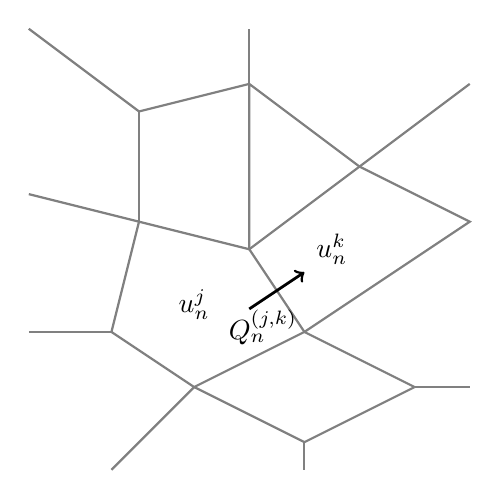
\begin{tikzpicture}[scale=0.35]
  %uncomment to see grid on which it was generated:
  %\draw[dotted,step=1.0,black,very thin] (0,0) grid (16,16);

    % exterior cell boundaries
  \draw[gray, thick] (3,0) -- (6,3);
  \draw[gray, thick] (0,5) -- (3,5);
  \draw[gray, thick] (0,10) -- (4,9);
  \draw[gray, thick] (0,16) -- (4,13);
  \draw[gray, thick] (4,13) -- (4,9);
  \draw[gray, thick] (4,13) -- (8,14);
  \draw[gray, thick] (8,14) -- (8,16);
  \draw[gray, thick] (12,11) -- (16,14);
  \draw[gray, thick] (10,5) -- (14,3);
  \draw[gray, thick] (10,1) -- (14,3);
  \draw[gray, thick] (14,3) -- (16,3);
  \draw[gray, thick] (6,3) -- (10,1);
  \draw[gray, thick] (10,0) -- (10,1);
  % interior cell boundaries
  \draw[gray, thick] (10,5) -- (8,8);
  \draw[gray, thick] (8,8) -- (12,11);



  % the free boundary is just like the other edges
  \draw[gray, thick] (6,3) -- (3,5) -- (4,9) -- (8,8) -- (8,14) --
              (12,11) -- (16,9) -- (10,5) -- cycle;
  % label some cell d.o.f.
  \draw (6,6) node {$u_n^j$};
  \draw (11,8) node {$u_n^k$};
  % show normal flux
  \def\xmid{9};
  \def\ymid{6.5};
  \def\dx{3/3};
  \def\dy{2/3};
  \draw[->,line width=1.0pt] (\xmid-\dx,\ymid-\dy) -- (\xmid+\dx,\ymid+\dy); % normal vector
  \draw (\xmid-\dx/2,\ymid-2*\dy) node {$Q_n^{(j,k)}$}; % label as flux
\end{tikzpicture}

\end{center}
\caption{Notation for an unstructured finite volume method for \eqref{eq:semimassconserve}.}
\label{fig:fvmesh-notation}
\end{figure}

We suppose the strong form \eqref{eq:semimassconserve} is discretized using finite volume ideas as shown in Figure \ref{fig:fvmesh-notation}.  The representative thickness $u_n^j$ in cell $j$ is given the usual finite volume definition as an average \cite{LeVeque2002}, as follows, and similarly $F_n^j$ denotes the average source term for the cell:
\begin{equation}
u_n^j \approx \frac{1}{|\omega_j|} \int_{\omega_j} u_n(x), \qquad F_n^j \approx \frac{1}{|\omega_j|} \int_{\omega_j} F_n(u_n,x).  \label{eq:fvthickness}
\end{equation}
(One may suppose these are computed by a quadrature scheme, but the details will not matter.)  The discrete (scalar) normal flux across the edge $(j,k)$, outward from cell $j$, is denoted
\begin{equation}
Q_n^{(j,k)} \approx \frac{1}{\ell_{(j,k)}} \int_{(j,k)} \bQ_n \cdot \bn_{(j,k)}. \label{eq:fvflux}
\end{equation}
Here $\bn_{(j,k)}$ denotes the unit normal vector to edge $(j,k)$ directed outward from $\omega_j$; thus $\bn_{(k,j)} = -\bn_{(j,k)}$.  We assume that these fluxes are approximated by some scheme, based on values $\{u_n^l\}$.  Again the details are not important here, but these discrete fluxes might be computed by upwinded and/or flux-limited schemes \cite{LeVeque2002} according to the functional form of the flux $\bQ_n$.

We assume that between any two adjacent \emph{fluid-filled} cells there is local conservation:
\begin{equation}
  u_n^j u_n^k > 0 \quad \implies \quad Q_n^{(k,j)}=-Q_n^{(j,k)}.  \label{eq:fvlocalconservation}
\end{equation}

FIXME: EXPLAIN THAT ONLY BACKWARD-EULER IS USED BUT IT IS NO RESTRICTION TO ASSUME \eqref{eq:fvmassconserve} ONLY FOR $u_n^j > 0$.  We also assume that if $u_n^j>0$ then the strong form single-time-step problem \eqref{eq:semimassconserve} is approximated by
\begin{equation}
\frac{u_n^j - u_{n-1}^j}{\Delta t_n} + \frac{1}{|\omega_j|} \sum_{k\in \mathcal{E}_j} Q_n^{(j,k)} \ell_{(j,k)} = F_n^j. \label{eq:fvmassconserve}
\end{equation}

Local discrete conservation statement \eqref{eq:fvlocalconservation} is completely standard, but the fluid-filled hypothesis is important.  We do \emph{not} expect discrete conservation, in the sense $Q_n^{(k,j)}=-Q_n^{(j,k)}$, at the free boundary.  This is because a flux scheme at the edge (face) of a fluid-free cell, facing a fluid-filled cell, cannot be expected to generate a flux which is compatible with the flow generating stresses (e.g.~body or boundary stresses) which yield nonzero fluxes in the neighboring fluid-filled cell.

Many schemes can be given interpretations \eqref{eq:fvthickness}--\eqref{eq:fvmassconserve}, including structured-grid (i.e.~uniform rectangular cell) finite difference \cite{Bueler2016,MortonMayers2005} and structured/unstructured finite volume \cite{LeVeque2002} schemes.  Regarding the sum in \eqref{eq:fvmassconserve}, recall that, at least heuristically, the divergence of a vector field $\bX$ is the limit of line (surface) integrals, $|R|^{-1} \int_{\partial R} \bX\cdot \bn \to \Div \bX$, where $R\subset \RR^d$ denotes a sequence of regions with Lipshitz boundary, enclosing and shrinking down to $x$, with outward unit normal vector $\bn$.  Though \eqref{eq:fvmassconserve} requires the discrete scheme to approximate such an integral, this form has great flexibility because of the many allowed meanings of approximations \eqref{eq:fvthickness} and \eqref{eq:fvflux}.

Pur finite volume description can instead be treated as a non-conforming Petrov-Galerkin finite element method for the variational inequality \eqref{eq:theVI}, with $A_n$ defined by \eqref{eq:defineAn}.  In that case the test functions are piecewise-constant and discontinuous along the edges of the cells $\omega_j$, as in a so-called ``finite volume element'' method \cite{Bueler2016,Cai1990,EwingLinLin2002}.  The cells $\omega_j$ would be geometrically ``dual'' to the elements in such a scheme (e.g.~\cite{Ringleretal2013}).

\subsection{The discrete-space ``shell error''}  \label{subsec:shellerror}  In the fully-discrete model we use a superscript ``$h$'' to denote the spatially-discrete version of integrated quantities.  Analogous to \eqref{eq:totalmassseries}, \eqref{eq:climateseries}, and \eqref{eq:retreatlossseries}, we define the time-series
\begin{align}
M_n^h &= \sum_j u_n^j |\omega_j|, \label{eq:fvtimeseriesdefn} \\
C_n^h &= \Delta t_n\!\!\sum_{\{j:u_n^j>0\}} F_n^j |\omega_j|,  \notag \\
R_n^h &= \sum_{\{j:u_n^j=0\}} u_{n-1}^j |\omega_j|.  \notag
\end{align}
Analogous to \eqref{eq:newbalance}, by \eqref{eq:fvmassconserve} we compute
\begin{align}
M_n^h - M_{n-1}^h &= \sum_{u_n^j>0} (u_n^j - u_{n-1}^j) |\omega_j| - \sum_{u_n^j=0} u_{n-1}^j |\omega_j| \notag \\
   &= - \Delta t_n\,\sum_{u_n^j>0}\, \sum_{(j,k)\in\mathcal{E}_j} Q_n^{(j,k)} \ell_{(j,k)} + \Delta t_n\,\sum_{u_n^j>0} F_n^j |\omega_j| - R_n^h \notag \\
   &= - \Delta t_n\,\sum_{u_n^j>0}\, \sum_{(j,k)\in\mathcal{E}_j} Q_n^{(j,k)} \ell_{(j,k)} + C_n^h - R_n^h.  \label{eq:fvnewbalance}
\end{align}

In the continuous-space version \eqref{eq:newbalance} we could eliminate the flux integral, but the discrete flux sum in \eqref{eq:fvnewbalance} is not zero.  However, local conservation \eqref{eq:fvlocalconservation} does reduce it to a sum over edges which have a positive-thickness cell on one side and a zero-thickness cell on the other.  We call this residual sum the \emph{shell error}:
\begin{equation}
S_n^h = \sum_{u_n^j>0}\, \sum_{(j,k)\in\mathcal{E}_j} Q_n^{(j,k)} \ell_{(j,k)} = \sum_{u_j^n > 0 \,\&\, (j,k)\in\mathcal{E}_j \,\&\, u_k^n = 0} Q_n^{(j,k)} \ell_{(j,k)} \label{eq:fvderiveshellerror}
\end{equation}
As suggested in Figure \ref{fig:fvmesh-shellerror}, $S_n^h$ is computed along the finite-volume approximation of the free boundary.  The quantity $S_n^h$ is an ``error'' in the sense that the continuous-space flux along the free-boundary would be zero because of flux conditions \eqref{eq:Qiscontinuous} and \eqref{eq:Qiszero}.

\begin{figure}[ht]
\begin{center}
% created by hand
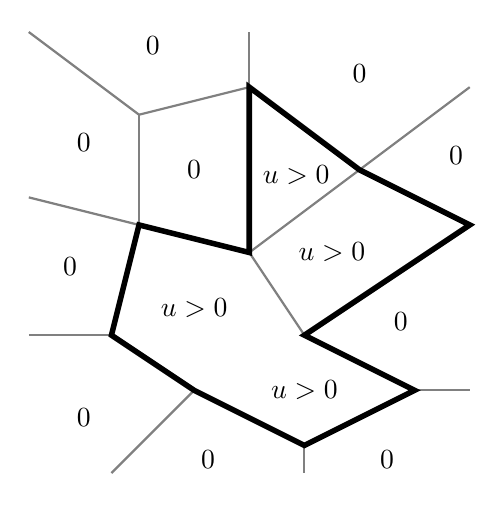
\begin{tikzpicture}[scale=0.35]
  %uncomment to see grid on which it was generated:
  %\draw[dotted,step=1.0,black,very thin] (0,0) grid (16,16);

    % exterior cell boundaries
  \draw[gray, thick] (3,0) -- (6,3);
  \draw[gray, thick] (0,5) -- (3,5);
  \draw[gray, thick] (0,10) -- (4,9);
  \draw[gray, thick] (0,16) -- (4,13);
  \draw[gray, thick] (4,13) -- (4,9);
  \draw[gray, thick] (4,13) -- (8,14);
  \draw[gray, thick] (8,14) -- (8,16);
  \draw[gray, thick] (12,11) -- (16,14);
  \draw[gray, thick] (10,5) -- (14,3);
  \draw[gray, thick] (10,1) -- (14,3);
  \draw[gray, thick] (14,3) -- (16,3);
  \draw[gray, thick] (6,3) -- (10,1);
  \draw[gray, thick] (10,0) -- (10,1);
  % interior cell boundaries
  \draw[gray, thick] (10,5) -- (8,8);
  \draw[gray, thick] (8,8) -- (12,11);



  % the free boundary is bold
  \draw[line width=2.0pt] (6,3) -- (3,5) -- (4,9) -- (8,8) -- (8,14) --
                          (12,11) -- (16,9) -- (10,5) -- (14,3) -- (10,1) -- cycle;
  % label cells with positive thickness
  \draw (6,6) node {$u>0$};
  \draw (11,8) node {$u>0$};
  \draw (9.7,10.8) node {$u>0$};
  \draw (10,3) node {$u>0$};
  % label cells with zero thickness
  \draw (2,2) node {$0$};
  \draw (1.5,7.5) node {$0$};
  \draw (2,12) node {$0$};
  \draw (4.5,15.5) node {$0$};
  \draw (6,11) node {$0$};
  \draw (12,14.5) node {$0$};
  \draw (15.5,11.5) node {$0$};
  \draw (13.5,5.5) node {$0$};
  \draw (13,0.5) node {$0$};
  \draw (6.5,0.5) node {$0$};
\end{tikzpicture}

\end{center}
\caption{The shell error $S_n^h$ is computed along those edges (strong line) where $u_n$ changes from positive (``$+$'') to zero (``$0$'').}
\label{fig:fvmesh-shellerror}
\end{figure}

At this point we can report computable time-series, namely $\{M_n^h,C_n^h,R_n^h,S_n^h\}$ which exactly balance in a fully-discrete free-boundary numerical computation:
\begin{equation}
  M_n^h = M_{n-1}^h + C_n^h - R_n^h - \Delta t_n\,S_n^h. \label{eq:fvfinalbalance}
\end{equation}

Recall that additional assumptions can show $R_n\to 0$ as $\Delta t_n\to 0$ (section \ref{sec:timeseries}).  FIXME also assert $S_n^h\to 0$ as $h\to 0$ \emph{if} free boundary well-behaved, which is beyond scope to show, but evidently $R_n^h + \Delta t_n\,S_n^h \to 0$ as $\Delta t_n\to 0$

\subsection{Fully-discrete explicit and semi-explicit schemes} \label{subsec:spaceexplicit}
FIXME  On the other hand, explicit and \emph{fully-discretized} numerical schemes are obviously in widespread use for solving first-order and even second-order PDE problems.  FIXME:  can be well-posed but regularity concerns different

\subsection{Newton-type methods} \label{subsec:newtonvi}  FIXME: mostly generalities \cite{Kelley2003}, but factor Jacobian into deriv of apparent stuff in \eqref{eq:theVI} and $\partial Q_n^j/\partial u_n^k$; equivalence of complementarity problems \cite{BensonMunson2006,BillupsMurty2000}; example in \cite{Bueler2016}

FIXME Condition (ii) could be summarized ``if $u_n^j>0$ then $G_j(u_n^J)=0$,'' using notation $u_n^J$ for a vector formed from all $u_n^j$ with $j\in J$, for some formula $G_j$ which records the residual of equation \eqref{eq:fvmassconserve}.  We also have constraint ``$u_n^j\ge 0$'' on the unknowns.  In these senses we are regarding the system of equations formed from conditions \eqref{eq:fvmassconserve} as combining to give a \emph{complementarity problem} \cite{BillupsMurty2000} of the form $u_j\ge 0$ and $G_j(u^J)\ge 0$ and $u_j G_j(u^J)=0$ for all $j\in J$


\section{Conclusion} \label{sec:conclusion}

Climate-scale fluid models generally claim exact discrete conservation as a goal \cite{Thuburn2008}, but apparently these claims are made in a context without free boundary.  Such climate models are ``multiphysics'' models which generally attempt to conserve masses of the phases of water (in particular) separately, as these phases have different physical properties relevant to earth system dynamics.  For example, snow and ice have higher albedo and lower density than the liquid ocean.

In many such models, one or more fluids or phases form a layer with a moving free boundary.  We believe that auditable mass conservation does not generally occur in these models, except perhaps through \emph{ad hoc} redistribution of mass, or \emph{ad hoc} discrete schemes to locally balance the books at the free boundary.  Discrete conservation is presumably recovered only in the temporal and spatial refinement limit in such models.

We identify the per time-step ``retreat area'' $\Omega_n^r$ and ``retreat loss'' $R_n$ for such models as important.  By definition $\Omega_n^r$ is the region where the fluid layer thickness is positive at the beginning of the time step, and, through flow and source terms, the thickness is zero at the end of the time step.  That is, fluid was completely lost at each location in the retreat area at some time during the time-step.  Even for well-behaved source terms (e.g.~smooth in time and space) and short time steps, the retreat area $|\Omega_n^r|$ can be of essentially arbitrary size.  For example, in a varying climate a large area of thin ice sheet or sea ice can melt, or a large area of a layer of surface water on ground can evaporate, and so on, during one time step.

In these terms we can answer question (ii) in the introduction more precisely:
\begin{quote}
  \emph{The retreat loss $R_n$ cannot be exactly balanced by a computable integral of the source term in the mass conservation equation during the time-step.}
\end{quote}
However, under reasonable stability assumptions on the solution to the weakly-posed single time-step problem,  $R_n$ goes to zero under temporal refinement even though the retreat area may not.  \emph{A priori} control on $R_n$ is possible under such assumptions.

The above conclusions apply in the time-semi-discretized case and thus are independent of particular spatial discretization schemes.  However, if space is discretized using a scheme that allows a finite volume (cell-wise) mass-conservation interpretation, we identify an additional, computable free-boundary-related conservation error.  This ``shell error'' $S_n$ occurs along that part of the free boundary where the flux would go to zero in the continuous case.  The shell errors go to zero under spatial refinement even when the time-step is not reduced.

With the conservation-correction time-series $\{R_n\}$ and $\{S_n\}$, a numerical model can ``balance the books'' exactly (i.e.~up to rounding error) in a manner which properly reflects the continuum model of the fluid layer.  Even without \emph{a priori} control, a user can then assess whether these free-boundary-related \emph{a posteriori} conservation errors are acceptably small.

We believe that avoidance of, or at least clearer understanding of, \emph{ad hoc} discrete schemes to maintain conservation at free boundaries will be possible once theoretical limits on discrete conservation are acknowledged, as here.  With the proposed corrections, for example, when a large area of ice sheet or sea-ice is modeled as melting entirely in a climate simulation model, that model can measure the amount of non-conservation of the mass of water in each phase, even if that model simply transfers the ice sheet retreat loss into the ocean.  More powerfully, adaptive time-stepping schemes can be modified to reduce the retreat loss, and adaptive mesh refinement or other paradigms can reduce the shell error below prescribed tolerances.  Climate models will then have better-quantified uncertainty for important mass transfers between component fluids of the climate.


%         References
\bibliographystyle{siamplain}
\bibliography{lc}


\appendix

\section{Inequalities for $p$-norms}   \label{app:pinequalities}  Versions of the inequalities in the next two Lemmas appear in the literature, at least as early as \cite{GlowinskiMarroco1975}, but here the results apply in $\RR^d$---contrast \cite{BarrettLiu1993,GlowinskiMarroco1975} for the $\RR^2$ case---and have complete proofs and explicit constants.  The proof follows and corrects \cite[Appendix A]{Peral1997}.

\begin{lemma}  \label{lem:pbiginequality}  If $p\ge 2$ and $x,y\in\RR^d$ then
\begin{equation}
\left(|x|^{p-2} x - |y|^{p-2} y\right)\cdot(x-y) \ge 2^{2-p} |x-y|^p. \label{eq:pbiginequality}
\end{equation}
\end{lemma}

\begin{proof}  The case where $x=0$ or $y=0$ is trivial, so assume, by swapping $x$ and $y$ as necessary, that $0 < |y| \le |x|$.  Define $t=|y|/|x|$ and $s = (x\cdot y)/(|x||y|)$ so that $0\le t \le 1$ and $|s|\le 1$.  Expand \eqref{eq:pbiginequality} and divide it by $|x|^p$, to get the equivalent statement
    $$1 - (t^{p-1}+t) s + t^p \ge 2^{2-p} \left(1 - 2 s t + t^2\right)^{p/2}.$$
Thus we need to prove that $2^{2-p}$ is a lower bound for
	$$f(t,s) = \frac{1 - (t^{p-1}+t) s + t^p}{\left(1 - 2 s t + t^2\right)^{p/2}}.$$
Note $s=1$ if and only if $x=y$, and in that case \eqref{eq:pbiginequality} is true.  We find a lower bound of $f$ on $(t,s) \in R=[0,1]\times[-1,1)$.  Note $1-2st+t^2 > 0$ on $ R$, so $f(t,s)$ is well-defined and differentiable on $R$.

Now, $f(t,-1) = \left(1 + t^{p-1}\right) / \left(1 + t\right)^{p-1}$ on $t\in[0,1]$.  Because $h(t)=t^{p-1}$ is convex for $p \ge 2$,
    $$\frac{1}{2^{p-1}} (1+t)^{p-1} = h(\tfrac{1}{2} 1 + \tfrac{1}{2} t) \le \tfrac{1}{2} h(1) + \tfrac{1}{2} h(t) = \tfrac{1}{2} (1 + t^{p-1}),$$
and thus $f(t,-1) \ge 2^{2-p}$.  On the other hand, a quick calculation shows
    $$\frac{\partial f}{\partial s} = \frac{t}{\left(1 - 2 s t + t^2\right)^{(p+2)/2}} g(t,s)$$
where
    $$g(t,s) = s(2-p) t (t^{p-2} + 1) + (p-1) (t^p+1) - t^{p-2} - t^2$$
is continuous on the closed rectangle $\bar R = [0,1]\times[-1,1]$.  We will show $g(t,s)\ge 0$ on $\bar R$, thus that $\partial f/\partial s \ge 0$ on $R$, and thus that $f(t,s)\ge f(t,-1) \ge  2^{2-p}$ on $R$.

Now,
    $$\frac{\partial g}{\partial s} = (2-p) t (t^{p-2} + 1) \le 0$$
on $\bar R$.  Define $G(t) = g(t,1)$.  We will show $G(t)\ge 0$ on $[0,1]$, thus that $g(t,s)\ge g(t,1)\ge 0$ on $\bar R$.  But
\begin{align*}
G(t) &\ge 0 &\iff && (2-p) t (t^{p-2} + 1) + (p-1) (t^p+1) - t^{p-2} - t^2 \ge 0 \\
          & &\iff && (p-1) (t-1) (t^{p-1}-1) \ge (t^{p-2} - t) (1 - t)  \\
          & &\iff && (p-1) (1 - t^{p-1}) \ge t^{p-2} - t.
\end{align*}
Note $(p-1) (1 - t^{p-1}) \ge 0$.  If $p\ge 3$ then $t^{p-2} - t \le 0$ so $G(t)\ge 0$ in that case.  On the other hand, if $2\le p < 3$ then
	$$\frac{t^{p-2} - t}{1 - t^{p-1}} = t^{p-2} \frac{1 - t^{3-p}}{1 - t^{p-1}} \le t^{p-2} \le 1 \le p-1$$
on $t\in[0,1)$, because $t^{p-1}\le t^{3-p}$ and thus $1 - t^{p-1} \ge 1 - t^{3-p}$.  But also $G(1)=0$, so $G(t)\ge 0$ on $[0,1]$. \end{proof}

\begin{lemma}  \label{lem:psmallinequality}  If $1<p\le 2$ and $x,y\in\RR^n$ then
\begin{equation}
\left(|x|^{p-2} x - |y|^{p-2} y\right)\cdot(x-y) \ge (p-1)\, |x-y|^2 \, \left(|x|+|y|\right)^{p-2}. \label{eq:psmallinequality}
\end{equation}
\end{lemma}

\begin{proof}  Assuming $x,y$ are not both zero, by symmetry (swapping $x$ and $y$) and homogeneity (replacing $x,y$ with $\lambda x,\lambda y$) we can assume $|x| = 1 \ge |y|$.  Furthermore, by choosing a basis of $\RR^d$ we can have $x=(1,0,\dots,0)$ and $y=(y_1,y_2,0,\dots,0)$ where $y_1^2+y_2^2 \le 1$.  In these terms, the inequality we seek to prove is
\begin{align*}
&\left(1 - (y_1^2+y_2^2)^{\frac{p-2}{2}} y_1\right) (1-y_1) + (y_1^2+y_2^2)^{\frac{p-2}{2}} y_2^2 \\
&\qquad\qquad \ge (p-1)\, \left((1-y_1)^2+y_2^2\right) \left(1 + \sqrt{y_1^2+y_2^2} \right)^{p-2}.
\end{align*}
(Compare equation (A.4) in \cite{Peral1997}.)  But
\begin{align*}
1 - (y_1^2+y_2^2)^{\frac{p-2}{2}} y_1
      &\ge \begin{cases} 1-y_1, & y_1 \le 0, \\
                        1-y_1^{p-1}, & 0 \le y_1 \le 1 \end{cases}\Bigg\}
      \ge (p-1) (1-y_1).
\end{align*}
(The lower case in the last inequality is easy to prove by the mean-value-theorem applied to $\varphi(t)=t^{p-1}$, for which $\varphi'(1)=p-1$ is the minimum value of the derivative on $t\in[0,1]$.)  Also noting $(y_1^2+y_2^2)^{\frac{p-2}{2}} \ge 1$ and $\left(1 + \sqrt{y_1^2+y_2^2} \right)^{2-p} \ge 1$, because $|y|\le 1$ and $p-2\le 0$, thus
\begin{align*}
&\frac{\left(1 - (y_1^2+y_2^2)^{\frac{p-2}{2}} y_1\right) (1-y_1) + (y_1^2+y_2^2)^{\frac{p-2}{2}} y_2^2}
      {\left((1-y_1)^2+y_2^2\right) \left(1 + \sqrt{y_1^2+y_2^2} \right)^{p-2}} \\
&\qquad \ge \frac{(p-1) (1-y_1)^2 + y_2^2}
      {(1-y_1)^2+y_2^2} \,  \left(1 + \sqrt{y_1^2+y_2^2} \right)^{2-p} \\
&\qquad \ge \frac{(p-1) (1-y_1)^2 + (p-1) y_2^2}{(1-y_1)^2+y_2^2} = p-1.
\end{align*}
This proves \eqref{eq:psmallinequality}. \end{proof}

We will also need the result of combining Lemma \ref{lem:psmallinequality}, a point-wise result, with integration over a set $\Omega$.

\begin{lemma} \label{lem:smallpbound}  Suppose $1<p\le 2$.  If $\Omega \subset \RR^d$ is measurable and if $\bu,\bv\in L^p(\Omega; \RR^m)$ for $m\ge 1$, then
\begin{equation}
    \int_\Omega \frac{|\bu-\bv|^p}{\left(|\bu|+|\bv|\right)^{2-p}} \ge \frac{\|\bu-\bv\|_{L^p(\Omega; \RR^m)}^2}{\big\||\bu|+|\bv|\big\|_{L^p(\Omega)}^{2-p}}. \label{eq:smallpbound}
\end{equation}
\end{lemma}

\begin{proof}  By H\"older inequality with $r=2/p$ and $s=2/(2-p)$, so $r^{-1}+s^{-1}=1$,
\begin{align*}
\int_\Omega |\bu - \bv|^p &= \int_\Omega \frac{|\bu-\bv|^p}{\left(|\bu|+|\bv|\right)^{p(2-p)/2}} \left(|\bu|+|\bv|\right)^{p(2-p)/2} \\
    &\le \left(\int_\Omega \frac{|\bu-\bv|^2}{\left(|\bu|+|\bv|\right)^{2-p}}\right)^{p/2} \left(\int_\Omega \left(|\bu|+|\bv|\right)^p\right)^{(2-p)/2},
\end{align*}
thus \eqref{eq:smallpbound}.
\end{proof}

Finally we recall the classical Poincar\'e inequality on the Sobolev space $W_0^{1,p}(\Omega)$.  This form, with an explicit but not optimal constant, is from \cite[section 7.8]{GilbargTrudinger2001}.

\begin{lemma} \label{lem:poincare}  If $\Omega\subset \RR^d$ is a bounded domain with volume $|\Omega|$, and if $1\le p<\infty$ then for all $u\in W_0^{1,p}(\Omega)$,
\begin{equation}
  \|u\|_{W^{1,p}(\Omega)}^p \le C(\Omega,p) \int_\Omega |\grad u|^p, \label{eq:poincare}
\end{equation}
where $C(\Omega,p)=1+(|\Omega|/\omega_d)^{p/d}$ and $\omega_d=(2 \pi^{d/2})/(d\,\Gamma(d/2))$ is the volume of the unit ball in $\RR^d$.
\end{lemma}


\section{Second-order Runge-Kutta time-discretization}  \label{app:rk2}  Section \ref{sec:strongform} describes the time semi-discretization of the continuum strong form \eqref{eq:massconserve}--\eqref{eq:constraint} using the $\theta$ method.  Such a one-stage time-discretization generates particular forms for the functions $\bQ_n(\bX,v,z)$ and $F_n(v,z)$ in equations \eqref{eq:semimassconserve}--\eqref{eq:semiconstraint}.  These functions determine the important variational inequality problem \eqref{eq:theVI}.  Here we illustrate how these functions can be generated for two particular Runge-Kutta (RK) schemes.  Generally one must solve multiple variational inequality problems \eqref{eq:theVI} during each time step of a multi-stage RK scheme.

For the $m$-dimensional ODE system
\begin{equation}
  \by' = \bbf(t,\by),  \label{eq:abstractODE}
\end{equation}
a two-stage RK scheme \cite{AscherPetzold1998} with time-step $h=\Delta t$ is given by
\begin{align}
  \by_{n,i} &= \by_{n-1} + h \sum_{j=1}^2 a_{ij} \bbf(t_{n-1} + \tau_j h, \by_{n,j}), \quad i=1,2, \label{eq:RK2} \\
      \by_n &= \by_{n-1} + h \sum_{i=1}^2 b_i \bbf(t_{n-1} + \tau_i h, \by_{n,i}). \notag
\end{align}
The constants $a_{ij},b_i,\tau_i$ depend upon the particular scheme.  \emph{Explicit} methods have $a_{ij}=0$ for $j\ge i$, i.e.~zeros on and above the diagonal in the Butcher tableau \cite{AscherPetzold1998}.  By definition, \emph{semi-implicit} methods have $a_{12}=0$.  We consider only explicit and semi-implicit methods.

\emph{Diagonally-implicit} RK (``DIRK'') methods are semi-implicit methods for which the diagonal entries $a_{ii}$ are independent of $i$, i.e.~$a_{11}=a_{22}$.  The accuracy of $s$-stage DIRK methods is limited to $p=s+1$ \cite{AscherPetzold1998}.  There exist strongly S-stable and stiffly-accurate \cite{AscherPetzold1998} DIRKs with $s$ stages and order of accuracy $p=s$ for $s=1,2,3$ \cite{Alexander1977}.  ``Strongly S-stable'' is also called ``stiff decay'' \cite{AscherPetzold1998}.  The strong stability properties of these DIRK methods are helpful for many applications addressed in the paper, namely cases where $\bq$ has a leading-order diffusion term.  (In such cases the $m$-dimensional method-of-lines ODE system is arbitrarily stiff under spatial refinement.)  Semi-implicit methods have the computational advantage that each stage generates an $m$-equation linear system, whereas general implicit RK schemes generate larger systems.  DIRK methods have the further advantage that the $m\times m$ matrix can be re-used at each stage of a time-step.  This matrix has stage-independent form $A = I - h a_{ii} J$ if the Jacobian $J$ is evaluated only at the start of the time step: $J = \frac{\partial \bbf}{\partial y}(t_{n-1},\by_{n-1})$.

Functions $\bQ_n$ and $F_n$ in \eqref{eq:functionalforms} appear in weak form \eqref{eq:theVI}.  Now, as an illustration, we compute these functions for the following two DIRK schemes: \emph{(a)} the $(s,p)=(1,2)$ A-stable scheme (implicit midpoint rule), and \emph{(b)} the unique strongly S-stable $(s,p)=(2,2)$ scheme for which $0\le \tau_i\le 1$ \cite{AscherPetzold1998}.
\renewcommand{\labelenumi}{\emph{(\alph{enumi})}}
\begin{enumerate}
\item The implicit midpoint rule has two stages, a backward Euler step of $\frac{1}{2} h$ followed by an explicit stage.  Using the notation $\tilde\by = \by_{n,2}$ the equations are
\begin{align}
\tilde\by &= \by_{n-1} + \tfrac{1}{2} h \bbf(t_{n-1}+\tfrac{1}{2}h,\tilde\by), \label{eq:impmida} \\
\by_n &= \by_{n-1} + h \bbf(t_{n-1}+\tfrac{1}{2}h,\tilde\by). \label{eq:impmidb}
\end{align}
Let $t_{n-1/2} = t_{n-1} + \tfrac{1}{2} \Delta t$.  Functions \eqref{eq:functionalforms} for the first stage \eqref{eq:impmida} are
  $$\tilde\bQ(\bX,v,x) = \tfrac{1}{2} \bq(\bX,v,x,t_{n-1/2}) \quad \text{and} \quad \tilde F(v,x) = \tfrac{1}{2} f(v,x,t_{n-1/2}).$$
Now let $\tilde u$ denote the weak solution to the first stage variational inequality problem.  The functions for the second stage \eqref{eq:impmidb} are $\bQ_n(\bX,v,x) = 0$ and
  $$\quad F_n(v,x) = f(\tilde u,x,t_{n-1/2}) - \Div \bq(\grad\tilde u,\tilde u,x,t_{n-1/2}).$$
Neither of these second-stage functions depend on the unknown $v$ because stage \eqref{eq:impmidb} is explicit.

\item The strongly S-stable $(2,2)$ scheme has equations
\begin{align}
\tilde\by &= \by_{n-1} + \alpha h \bbf(\tilde t,\tilde\by), \label{eq:sstabledirka} \\
\by_n &= \by_{n-1} + (1-\alpha) h \bbf(\tilde t,\tilde\by) + \alpha h \bbf(t_n,\by_n). \label{eq:sstabledirkb}
\end{align}
where $\alpha = (2-\sqrt{2})/2$, $\tilde\by = \by_{n,1}$, and $\tilde t = t_{n-1} + \alpha h$.  The functions \eqref{eq:functionalforms} for the first stage \eqref{eq:sstabledirka} are
  $$\tilde\bQ(\bX,v,x) = \alpha \bq(\bX,v,x,\tilde t) \quad \text{and} \quad \tilde F(v,x) = \alpha f(v,x,\tilde t).$$
If $\tilde u$ denotes the weak solution to the first stage variational inequality problem then the functions for the second stage \eqref{eq:sstabledirkb} are $\bQ_n(\bX,v,x) = \alpha \bq(\bX,v,x,t_n)$ and
   $$F_n(v,x) = (1-\alpha) f(\tilde u,x,\tilde t) + \alpha f(v,x,t_n) - (1-\alpha) \Div \bq(\grad\tilde u,\tilde u,x,\tilde t).$$
\end{enumerate}

\end{document}
